\documentclass[a4paper,12pt]{article}

\usepackage{tocloft}
\usepackage[utf8]{inputenc}
\usepackage[T1]{fontenc}
\usepackage[french]{babel}
\usepackage{tabularx}
\usepackage{amsmath}
\usepackage{graphicx}
\usepackage{float}
\usepackage{subcaption}
\usepackage{hyperref}
\usepackage{cite}
\usepackage{url}
\usepackage{listings}
\usepackage{xcolor}
\usepackage{csquotes}
\usepackage{times}
\usepackage{setspace}
\usepackage{amsmath}
\usepackage{amssymb}
\usepackage[top=2cm, bottom=2cm, left=2cm, right=2cm]{geometry}

\setlength{\parindent}{0pt}
\setlength{\parskip}{0.5em}
\setstretch{1.5}

\newcommand{\fonctionLogistique}[1]{%
    \frac{1}{1 + \exp\left(-#1\right)}%
}

\newcommand{\optimisationSVM}{%
    \min_{w, b} \ \frac{1}{2} \|w\|^2 \quad \text{s.c.} \quad y_i(w^T x_i + b) \geq 1
}

\newcommand{\noyauRBF}[2]{%
    \exp\left(-\gamma \|#1 - #2\|^2\right)
}

\newcommand{\voteMajoritaire}[1]{%
    \text{mode}\left(#1\right)
}

\newcommand{\fonctionObjectifXGBoost}{%
    \mathcal{L}(t) = \sum_{i=1}^n l\bigl(y_i, \hat{y}_i^{(t-1)} + f_t(x_i)\bigr) + \Omega(f_t)
}

\newcommand{\regulXGBoost}{%
    \Omega(f) = \gamma T + \frac{1}{2} \lambda \sum_j w_j^2
}


\begin{document}

\pagenumbering{roman}
\pagestyle{plain}

% ===== PAGE DE GARDE =====
\begin{titlepage}
\thispagestyle{empty}
\begin{titlepage}
    \centering
    \small
    
    
\includegraphics[width=4cm]{img/INSI.png}\\[0.3cm]
    \textbf{INSI}\\
    \rule{0.5\textwidth}{0.4pt}\\[0.2cm]

    \textbf{INSTITUT NATIONAL SUPERIEUR D'INFORMATIQUE}\\[0.5cm]

    \textbf{Mémoire de projet en vue de l’obtention du diplôme de Licence}\\[0.3cm]

    Domaine : Sciences et Technologie \\
    Mention : Informatique \\
    Parcours : Intelligence Artificielle et Data \\[0.5cm]

    \textbf{Par :}
         ANDRIANJAKA Idris Tovonirina \\[0.5cm]

    \textbf{\large  Mise en place d'un 
système intelligent pour l'intelligence 
concurrentielle et l'aide à la décision 
commerciale}\\[0.5cm]

    Date du début et fin du projet : \\
    1 Septembre 2026 - 1 Décembre 2026 \\[0.5cm]

    Soutenu le 05 Août 2025, devant la commission d'examen composée de :\\[0.3cm]

    Président du Jury : \\
    Dr RAJAOSOLOMANANTENA Haingonirina Ignace \\[0.3cm]

    Examinateur :\\
    Mr RASOLOFOMANANA Tolotra Iarivony Nirina \\[0.3cm]

    Encadreur Academique :\\
    Dr RAMASONDRANO Andriamanjaka\\
    [0.3cm]

    Encadreur Professionel:\\
    Mr Ny Hakanto Ratrema

    \vfill

    \hfill \textbf{Année Universitaire : 2025-2026}
\end{titlepage}

\end{titlepage}
\newpage
\thispagestyle{empty}
\mbox{}
\newpage

% ===== RESUME / ABSTRACT (a activer quand les fichiers existeront) =====
% \input{resume}
% \newpage
% \input{abstract}
% \newpage

\tableofcontents
\newpage

\renewcommand{\listfigurename}{Listes des Figures}
\listoffigures
\newpage

\listoftables
\newpage

\newpage
\pagenumbering{arabic}
\setcounter{page}{1}

% ===== CORPS DU MEMOIRE (a activer partie par partie) =====
\section{Introduction Générale}

\subsection{Contexte général}

Dans un secteur des services numériques de plus en plus concurrentiel, la capacité d'une entreprise à
positionner correctement son offre commerciale constitue un avantage stratégique déterminant. Les
entreprises de développement web et mobile évoluent dans un marché où les prix pratiqués, la qualité
perçue des prestations et la réputation des concurrents évoluent en permanence. Or, la collecte et
l'exploitation de ces informations reposent encore, dans la majorité des cas, sur des démarches manuelles,
ponctuelles et peu structurées.

Le développement récent des techniques d'intelligence artificielle générative, et en particulier des
architectures de \textit{Retrieval-Augmented Generation} (RAG), ouvre de nouvelles perspectives pour
automatiser la collecte, la structuration et l'exploitation de données non structurées issues du web. Combinées
à des techniques de traitement automatique du langage naturel (NLP) telles que l'analyse de sentiment,
ces approches permettent de transformer des données brutes --- prix affichés, avis clients --- en
informations directement exploitables par les équipes commerciales.

C'est dans ce contexte que s'inscrit le stage de fin d'études réalisé au sein d'ICHTUS IT, entreprise
spécialisée dans le développement de plateformes web et d'applications mobiles.

\subsection{Problématique et enjeux}

Aujourd'hui, ICHTUS IT ne dispose d'aucun outil centralisant les données tarifaires et les avis clients de
ses concurrents. Chaque commercial doit effectuer ses propres recherches ponctuelles, sans historique ni
vision d'ensemble sur le positionnement du marché. Cette absence d'outillage ralentit le chiffrage des
offres et prive l'équipe commerciale d'arguments de vente construits sur des données réelles.

La problématique de ce mémoire peut donc être formulée ainsi : \textit{comment automatiser la collecte des
données tarifaires et des avis clients des entreprises concurrentes, et les rendre exploitables en temps réel
via un agent conversationnel, pour permettre à l'équipe commerciale de prendre des décisions de pricing et
de prospection plus rapides et mieux argumentées ?}

Cette problématique soulève des enjeux à plusieurs niveaux :
\begin{itemize}
    \item \textbf{Enjeux scientifiques et techniques} : concevoir un pipeline robuste de collecte de données
    web non structurées, une architecture de recherche vectorielle performante, et un système de
    classification de sentiment fiable en l'absence de données annotées.
    \item \textbf{Enjeux industriels} : réduire le temps de recherche manuelle des commerciaux et fiabiliser
    la prise de décision en matière de pricing.
    \item \textbf{Enjeux socio-économiques} : renforcer la compétitivité d'ICHTUS IT sur son marché grâce à
    une meilleure connaissance de son environnement concurrentiel.
\end{itemize}

\subsection{Objectifs du stage et du mémoire}

Ce stage vise à concevoir et développer un système capable de :
\begin{itemize}
    \item collecter automatiquement les prix pratiqués par les entreprises concurrentes du secteur du
    développement web et mobile ;
    \item mettre ces données à disposition de l'équipe commerciale via un agent conversationnel interrogeable
    en langage naturel ;
    \item analyser les avis clients laissés sur les concurrents afin d'en extraire automatiquement le
    sentiment global ainsi que les points forts et points faibles récurrents.
\end{itemize}

L'objectif du mémoire est, quant à lui, de documenter la démarche scientifique et technique ayant permis
d'aboutir à ce système, de la revue de littérature jusqu'à l'évaluation des résultats obtenus.

\subsection{Hypothèses et questions de recherche}

Ce travail repose sur les hypothèses suivantes :
\begin{itemize}
    \item il est possible de collecter de manière automatisée et fiable des données tarifaires et des avis
    clients publiés en ligne par des entreprises concurrentes, malgré l'hétérogénéité de leur présentation ;
    \item une architecture RAG appuyée sur une recherche par similarité vectorielle permet de restituer une
    information de marché pertinente et à jour, sans nécessiter de réentraînement du modèle de langage ;
    \item une analyse de sentiment en \textit{zero-shot}, sans fine-tuning ni jeu de données annoté, offre une
    précision suffisante pour être exploitée par des utilisateurs non techniques.
\end{itemize}

Ces hypothèses guident les questions de recherche suivantes : dans quelle mesure un pipeline ETL appliqué à
des données web non structurées permet-il d'alimenter un système d'aide à la décision fiable ? Et comment
combiner recherche vectorielle et extraction de sentiment pour produire une réponse à la fois quantitative
et qualitative sur le positionnement des concurrents ?

\subsection{Méthodologie générale adoptée}

La démarche suivie s'articule en trois grandes phases correspondant aux trois couches du système développé :

\begin{enumerate}
    \item une phase de \textbf{collecte de données}, reposant sur un scraping intelligent automatisé
    (ScrapeGraphAI) des pages de tarifs et d'avis clients, suivie d'un pipeline de transformation
    (parsing, structuration) inspiré des démarches ETL classiques ;
    \item une phase de \textbf{stockage et de traitement}, avec une base de données Supabase/PostgreSQL
    indexée pour la recherche sémantique grâce à l'extension \texttt{pgvector} ;
    \item une phase d'\textbf{intelligence artificielle}, combinant un système de RAG pour l'interrogation en
    langage naturel du marché, et un module d'analyse de sentiment basé sur un grand modèle de langage en
    extraction \textit{zero-shot}.
\end{enumerate}

Cette méthodologie est détaillée et justifiée dans les chapitres consacrés à l'état de l'art et à la
méthodologie du présent mémoire.

\subsection{Organisation du mémoire}

Ce mémoire s'organise de la manière suivante. Le chapitre 2 présente l'établissement académique
d'origine, l'INSI. Le chapitre 3 présente l'entreprise d'accueil, ICHTUS IT. Le chapitre 4 expose le
cadrage du projet, les besoins identifiés et les contraintes rencontrées. Le chapitre 5 propose une revue
de la littérature scientifique et technique relative au sujet traité. Le chapitre 6 détaille la méthodologie
adoptée. Les chapitres 7 et 8 présentent respectivement l'exploration et la préparation des données, puis
la modélisation et les expérimentations menées. Le chapitre 9 décrit le déploiement du système sous forme
de démonstrateur. Le chapitre 10 propose une discussion critique des résultats obtenus, avant que le
chapitre 11 n'expose les limites du travail et les perspectives envisagées. Le mémoire se conclut par une
synthèse générale des apports scientifiques, techniques et professionnels de ce stage.
\newpage
% \input{INSI}
% \newpage
\section{Cadrage}

Le secteur du développement web et mobile, en particulier dans un contexte de forte concurrence
entre agences et sociétés de services numériques, fait face à un défi récurrent : la difficulté à connaître
précisément le positionnement tarifaire et la réputation des entreprises concurrentes. Cette problématique
revêt une importance stratégique, car une méconnaissance du marché peut conduire à un mauvais
positionnement commercial, à des offres mal chiffrées, voire à une perte de compétitivité face à des
concurrents mieux informés.

Les défis spécifiques rencontrés dans ce domaine incluent :
\begin{itemize}
    \item \textbf{Dispersion et hétérogénéité de l'information} : les prix et les avis clients des concurrents
    sont disséminés sur de multiples supports (sites vitrines, plateformes d'avis, réseaux sociaux), sans
    format ni structure commune, ce qui rend leur collecte manuelle longue et peu fiable.
    \item \textbf{Évolution constante du marché} : les tarifs pratiqués et la réputation des concurrents évoluent
    en continu, rendant obsolète toute veille ponctuelle réalisée à un instant donné.
    \item \textbf{Absence d'outillage adapté} : les équipes commerciales ne disposent d'aucun outil centralisé
    leur permettant d'interroger rapidement ces informations au moment de chiffrer une offre ou de
    préparer une prospection.
\end{itemize}

Ce projet vise à développer un système capable d'automatiser la collecte de ces données, de les
structurer et de les rendre accessibles à travers un agent conversationnel intelligent, en s'appuyant sur des
techniques d'intelligence artificielle générative et de traitement automatique du langage. L'objectif est de
substituer une démarche manuelle et ponctuelle par une veille continue, structurée et directement
exploitable par des utilisateurs non techniques.

\subsection{Besoins exprimés et opportunités identifiées}

ICHTUS IT a exprimé le besoin de disposer d'une vision consolidée et actualisée du marché sur lequel elle
évolue, sans mobiliser de ressources humaines supplémentaires pour cette veille. Concrètement, l'entreprise
souhaite que ses commerciaux puissent, en une question posée en langage naturel, obtenir à la fois le
positionnement tarifaire d'un ou plusieurs concurrents et une synthèse qualitative de leur réputation
client. Cette opportunité s'inscrit dans la volonté plus large de l'entreprise d'outiller ses équipes
commerciales avec des solutions basées sur la donnée plutôt que sur l'intuition.

\subsection{Données disponibles}

Les données mobilisées dans ce projet proviennent exclusivement de sources publiquement accessibles sur
le web : pages tarifaires publiées par les entreprises concurrentes, et avis clients publiés sur des plateformes
publiques. Ces données sont hétérogènes par nature (texte libre, tableaux de prix, notes chiffrées) et
nécessitent un travail de structuration avant exploitation. Le volume de données dépend directement du
nombre de concurrents suivis et de la fréquence de rafraîchissement du scraping, ce volume étant appelé à
croître progressivement au fil du stage à mesure que de nouveaux concurrents sont ajoutés au périmètre de
veille.

\subsection{Contraintes}

Plusieurs contraintes encadrent la réalisation de ce projet :
\begin{itemize}
    \item \textbf{Contraintes légales} : seules des données publiquement accessibles sont collectées, dans le
    respect des conditions d'utilisation des sites concernés et des principes du RGPD, notamment en évitant
    toute collecte de données à caractère personnel identifiable.
    \item \textbf{Contraintes techniques liées à la structure des sites cibles} : la majorité des sites de
    concurrents ciblés sont construits avec des frameworks JavaScript modernes (rendu côté client), ce qui
    rend leur contenu inaccessible à un scraping classique basé sur des bibliothèques comme BeautifulSoup,
    limitées à l'analyse du HTML statique. Cette contrainte impose le recours à un outil de scraping capable
    d'interpréter le rendu dynamique des pages, en l'occurrence ScrapeGraphAI, qui combine navigation
    automatisée et extraction pilotée par un modèle de langage.
    \item \textbf{Contraintes de coût} : le recours à une solution de scraping basée sur des appels à une API
    (ScrapeGraphAI) engendre un coût par requête, ce qui impose d'optimiser la fréquence de rafraîchissement
    des données et de limiter le nombre d'appels redondants, plutôt que de scraper en continu l'ensemble des
    sources suivies.
    \item \textbf{Contraintes métier} : le système doit rester utilisable par des profils non techniques ; toute
    réponse fournie par l'agent conversationnel doit donc être claire, synthétique et directement actionnable
    par un commercial.
    \item \textbf{Contraintes temporelles} : le développement, l'expérimentation et l'évaluation du système
    doivent être réalisés dans le cadre du stage, ce qui impose de prioriser un périmètre fonctionnel réaliste.
\end{itemize}

\subsection{Périmètre géographique et utilisateurs}

Le périmètre retenu est la \textbf{métropole lilloise et ses environs} (Lille, communes limitrophes,
Hauts-de-France proches), sur des prestations de \textbf{développement web et mobile}. Les utilisateurs
cibles sont les commerciaux et l'encadrement commercial d'ICHTUS IT. On distingue les concurrents
\textit{implantés ou suivis} dans ce périmètre (présents en base) des acteurs simplement cités hors zone,
pour lesquels le système doit s'abstenir ou signaler une couverture insuffisante.

\subsection{Objectifs mesurables et questions techniques}

Les objectifs du projet sont formulés de manière vérifiable :
\begin{itemize}
    \item \textbf{O1 --- Collecte et structuration.} Disposer d'une base de concurrents avec fiches prix
    exploitables (cible observée : environ 69 fiches après filtrage qualité) et d'analyses de sentiment
    pour une part significative de ces fiches.
    \item \textbf{O2 --- Interrogation en langage naturel.} Permettre à un commercial d'obtenir, via une
    question en français, une réponse fondée uniquement sur les fiches retrouvées (architecture RAG).
    \item \textbf{O3 --- Robustesse des gardes-fous.} Rejeter ou signaler les questions hors sujet, hors
    zone géographique et hors couverture métier.
    \item \textbf{O4 --- Évaluation.} Séparer un jeu de développement et un jeu de test indépendant ;
    mesurer le comportement de retrieval et compléter par une grille humaine de qualité de réponse.
\end{itemize}

Questions techniques / hypothèses de travail :
\begin{itemize}
    \item \textbf{Q1.} Un RAG sur fiches structurées (prix + avis) suffit-il à produire des réponses
    commercialement utiles, sans fine-tuning d'un modèle de langue ?
    \item \textbf{Q2.} Un seuil de similarité et un filtre géographique structurel réduisent-ils les
    réponses hors périmètre par rapport à un prompt seul ?
    \item \textbf{Q3.} Une analyse de sentiment zero-shot par LLM est-elle suffisamment fiable, sur un
    échantillon annoté, pour enrichir les fiches sans modèle supervisé dédié ?
\end{itemize}

\subsection{Définition des indicateurs de performance (KPI)}

Afin d'évaluer objectivement la réussite du projet, les indicateurs suivants sont retenus :
\begin{itemize}
    \item \textbf{Couverture de la veille} : nombre de concurrents et de sources suivis de manière automatisée.
    \item \textbf{Fraîcheur des données} : délai moyen entre la mise à jour d'une information chez un
    concurrent et sa disponibilité dans le système (à mesurer ou à déclarer non mesuré si hors délai du stage).
    \item \textbf{Comportement de retrieval du RAG} : taux de questions pertinentes avec résultat, taux de
    rejet hors sujet, Hit Rate@$k$ / MRR sur vérité terrain nominative (diagnostics de recherche).
    \item \textbf{Qualité des réponses générées} : grille humaine (sources, montants/devises, fidélité,
    complétude, abstention, utilité commerciale).
    \item \textbf{Qualité de l'analyse de sentiment} : comparaison à une annotation manuelle de référence
    sur un échantillon d'avis (macro-F1 / matrice de confusion).
    \item \textbf{Gain de temps commercial} : réduction estimée du temps de recherche d'information par
    rapport à une veille manuelle (avec le référent métier si disponible).
\end{itemize}

\subsection{Cahier des charges}

\subsubsection{Exigences fonctionnelles}

\begin{itemize}
    \item \textbf{EF1.} Collecter et mettre à jour les données tarifaires et d'avis de concurrents web/mobile
    du périmètre depuis des sources publiques (Clutch, La Fabrique du Net).
    \item \textbf{EF2.} Stocker les données dans une base relationnelle (Supabase/PostgreSQL) avec historique
    des changements de prix.
    \item \textbf{EF3.} Produire une analyse de sentiment structurée (global, score, points forts/faibles)
    à partir des avis.
    \item \textbf{EF4.} Indexer les fiches en embeddings et répondre à des questions en français via RAG,
    en citant les sources utilisées.
    \item \textbf{EF5.} Appliquer des gardes-fous : hors sujet, hors zone, hors couverture, seuil de
    similarité.
    \item \textbf{EF6.} Exposer le pipeline de façon testable en ligne de commande (et, si le calendrier le
    permet, via une API / interface).
\end{itemize}

\subsubsection{Exigences non fonctionnelles}

\begin{itemize}
    \item \textbf{ENF1 --- Utilisabilité.} Réponses en français, synthétiques, actionnables par un
    commercial non technique.
    \item \textbf{ENF2 --- Fidélité.} Interdiction d'inventer des tarifs ou avis absents des fiches ;
    signaler les informations manquantes.
    \item \textbf{ENF3 --- Coût.} Limiter les appels API (scraping, embeddings, LLM) ; privilégier Gemini
    en développement et un modèle plus capable en démonstration si besoin.
    \item \textbf{ENF4 --- Reproductibilité.} Documenter modèles, paramètres, version du corpus, scripts
    d'évaluation et séparation développement / test.
    \item \textbf{ENF5 --- Conformité.} Données publiques uniquement ; pas de données personnelles
    identifiables ; respect des conditions d'usage des sources.
\end{itemize}

\subsubsection{Hors périmètre (Éval~1 / stage)}

Sauf réalisation explicite et évaluée : génération automatisée de leads commerciaux, pricing
prescriptif (recommandation du prix ICHTUS), couverture nationale hors métropole lilloise, fine-tuning
d'un modèle de langue from scratch.

\subsubsection{Critères d'acceptation}

Un critère est \textbf{satisfait} uniquement s'il est démontrable (script, capture, tableau de résultats
ou annotation).

\begin{table}[H]
\centering
\begingroup
\setstretch{1.15}
\small
\begin{tabularx}{\textwidth}{|c|X|X|}
\hline
\textbf{ID} & \textbf{Critère} & \textbf{Preuve attendue} \\
\hline
CA1 & Au moins une base de fiches prix indexées (embeddings non nuls)
& Comptage SQL / script ; $n$ fiches documenté \\
\hline
CA2 & Une question nominative ramène la fiche attendue dans le TOP-$k$
& Hit Rate sur jeu de test / vérité terrain \\
\hline
CA3 & Une question hors sujet ne ramène pas de fiche concurrent
& Scénarios hors sujet du protocole d'évaluation \\
\hline
CA4 & Une question hors zone (ex.\ Tokyo) est bloquée ou signalée
& Filtre géographique + scénario de test \\
\hline
CA5 & Les montants cités dans la réponse sont présents dans les sources
& Grille humaine (exactitude montants/devises) \\
\hline
CA6 & Jeu de développement distinct du jeu de test ; config figée avant le test
& Fichiers \texttt{dev\_questions} / \texttt{test\_questions} + config figée \\
\hline
CA7 & Échantillon d'avis annoté pour évaluer le sentiment (même réduit)
& Règles d'annotation + scores (ex.\ macro-F1) \\
\hline
CA8 & Pipeline exécutable par un tiers autorisé
& README : installation, variables, commandes de test \\
\hline
\end{tabularx}
\endgroup
\caption{Critères d'acceptation du système (Évaluation~1 et suivi)}
\label{tab:criteres_acceptation}
\end{table}

\subsection{Importance des solutions apportées}

\subsubsection{Amélioration de la prise de décision commerciale}

L'automatisation de la veille concurrentielle permet de transformer des données dispersées et non
structurées en informations directement exploitables. En combinant recherche vectorielle et analyse de
sentiment, le système proposé offre une vision à la fois quantitative (positionnement tarifaire) et
qualitative (perception client) du marché, permettant aux commerciaux d'argumenter leurs offres sur des
bases factuelles plutôt que sur des impressions.

L'impact de cette solution dépasse le cadre strictement opérationnel : en réduisant le temps consacré à la
recherche manuelle d'informations, elle libère du temps commercial pouvant être réinvesti dans la relation
client. Elle contribue également à une meilleure réactivité de l'entreprise face aux évolutions du marché.

\subsubsection{Objectifs et impacts attendus}

Les principaux objectifs de ce projet consistent à développer un système fonctionnel de veille
concurrentielle automatisée, adapté aux spécificités du secteur du développement web et mobile. Ce
développement s'accompagne d'une exigence de fiabilité, tant dans la collecte des données que dans la
pertinence des réponses fournies par l'agent conversationnel.

L'évaluation rigoureuse du système, à travers les indicateurs définis précédemment, constitue un axe
essentiel du projet, permettant de mesurer objectivement son apport par rapport à une démarche de veille
manuelle. Enfin, ce projet ambitionne de constituer un socle réutilisable, l'architecture développée pouvant
être étendue à d'autres secteurs d'activité ou à d'autres types de données concurrentielles au sein de
l'entreprise.
\newpage
\section{État de l'Art}

\subsection{Méthodologie de la revue de littérature}

Cette revue de l'état de l'art a été conduite en croisant deux types de sources, conformément aux exigences
méthodologiques d'un mémoire de licence en intelligence artificielle et data : des sources bibliographiques
scientifiques (articles évalués par les pairs, prépublications arXiv, actes de conférences ACM/IEEE,
chapitres Springer) et des sources webographiques (blogs techniques spécialisés, dépôts GitHub de
référence, livres blancs d'éditeurs). Les bases consultées incluent arXiv, Springer Link, ScienceDirect et
ResearchGate. Les mots-clés de recherche combinaient les trois axes techniques du projet : retrieval-augmented
generation, analyse de sentiment par modèles de langage, et web scraping appliqué à l'intelligence
concurrentielle.

\subsection{Études bibliographiques}

\subsubsection{Retrieval-Augmented Generation (RAG)}

Le paradigme RAG a été introduit par Lewis et al. (2020) \cite{lewis2020} dans un article fondateur présenté
à NeurIPS, qui propose de coupler un modèle génératif à un mécanisme de récupération d'information externe
afin de pallier les limites des modèles de langage purement paramétriques : hallucinations, obsolescence des
connaissances et absence d'expertise de domaine spécifique. Cette approche a depuis fait l'objet de
nombreuses synthèses. Wu et al. (2024) \cite{wu2024} proposent une revue systématique centrée sur les
mécanismes de récupération et de fusion (query-based, logits-based, latente, paramétrique), et établissent
une taxonomie comparant ces approches selon leur accessibilité, leur efficacité et leurs cas d'usage. Yu et
al. (2024) \cite{yu2024} se concentrent quant à eux sur l'évaluation des systèmes RAG et proposent un cadre
unifié (Auepora) structurant les métriques autour de trois axes : la pertinence de la récupération,
l'exactitude de la génération et la fidélité aux sources récupérées.

Plusieurs travaux récents traitent des limites intrinsèques du RAG de base et proposent des correctifs
pertinents pour ce projet. Yan et al. (2024) \cite{yan2024} introduisent le Corrective RAG, qui ajoute une
étape de vérification de la pertinence des documents récupérés avant leur transmission au modèle générateur
--- une logique proche du seuil de confiance mis en œuvre dans ce projet. Xu et al. (2024) \cite{xu2024},
lors de SIGIR 2024, montrent l'intérêt de coupler RAG et graphes de connaissances pour des cas d'usage de
service client, un contexte proche de l'assistance commerciale visée ici. Xue et al. (2024) \cite{xue2024}
documentent par ailleurs des vulnérabilités de sécurité propres aux systèmes RAG (BadRAG), rappelant que la
fiabilité de ces architectures reste un sujet de recherche actif plutôt qu'un problème résolu.

\subsubsection{Analyse de sentiment par grands modèles de langage}

L'analyse de sentiment a longtemps reposé sur des modèles supervisés entraînés spécifiquement sur la tâche
(SVM, puis modèles Transformer de type BERT ou FinBERT). L'émergence des grands modèles de langage
généralistes a introduit un nouveau paradigme, le zero-shot, où le modèle classe le sentiment sans exemple
d'entraînement spécifique. Simmering et Huoviala (2023) \cite{simmering2023} comparent GPT-4 et GPT-3.5 en
zero-shot, few-shot et fine-tuné sur une tâche d'analyse de sentiment par aspect (ABSA) : le modèle fine-tuné
atteint un score F1 état de l'art de 83,8, mais au prix d'un coût d'inférence largement supérieur ; les
auteurs concluent que des prompts détaillés améliorent significativement les performances en zero-shot et
few-shot, rendant cette approche viable en l'absence de données annotées.

Cette conclusion est corroborée par une étude publiée dans JMIR Formative Research (2025) évaluant GPT-4 sur
des données de santé publique : la précision en configuration zero-shot atteint déjà 92\,\% pour le sentiment
positif, avec une amélioration marginale seulement en few-shot, ce qui suggère que les grands modèles
récents disposent d'une capacité de classification de sentiment déjà robuste sans exemples. Vamvourellis et
Mehta (2025) \cite{vamvourellis2025}, dans une étude menée chez BlackRock sur le sentiment financier,
comparent plusieurs LLM propriétaires en zero-shot face à des modèles FinBERT spécialisés fine-tunés, et
notent que les stratégies de raisonnement explicite (chain-of-thought) n'améliorent pas systématiquement
l'alignement avec l'annotation humaine, en particulier sur les cas peu ambigus. Une synthèse plus large
portant sur 13 tâches et 26 jeux de données (citée dans une revue de 2026 sur l'analyse de sentiment
appliquée aux critiques de films) confirme que les LLM en zero-shot restent compétitifs sur des tâches de
classification simple, mais restent en retrait des modèles spécialisés fine-tunés sur les tâches nécessitant
une compréhension fine de phénomènes de sentiment complexes. Beno (2025) \cite{beno2025} montre enfin qu'une
approche hybride combinant un modèle spécialisé (ELECTRA) et un LLM généraliste (GPT-4o) permet d'obtenir le
meilleur rapport coût/performance, ouvrant une piste d'amélioration pour des travaux futurs.

\subsubsection{Web scraping et intelligence concurrentielle}

La littérature académique portant spécifiquement sur le web scraping appliqué à l'intelligence
concurrentielle reste comparativement restreinte. Un chapitre publié chez Springer Nature (2025)
\cite{springer2025} propose un état de l'art accompagné d'une étude de cas démontrant que l'intégration du
web scraping dans une stratégie d'entreprise améliore la compréhension du marché ; les auteurs soulignent
également les défis inhérents à cette pratique (structuration des données hétérogènes, maintenance des
extracteurs face aux évolutions des sites) et évoquent la contribution potentielle de l'intelligence
artificielle pour renforcer ces systèmes --- un argument central pour justifier le recours à un extracteur
piloté par IA plutôt qu'à des sélecteurs CSS statiques dans ce projet. Une revue bibliométrique de 2025,
fondée sur l'analyse de 567 publications \cite{bibliometrique2025}, confirme la croissance rapide mais
récente du champ de recherche combinant web scraping et modèles d'IA pour des applications d'entreprise, ce
qui situe ce projet dans un domaine de recherche encore émergent académiquement, malgré une pratique déjà
répandue dans l'industrie.

\subsection{Études webographiques}

En complément des sources académiques, plusieurs ressources techniques non évaluées par les pairs ont été
consultées pour leur pertinence opérationnelle immédiate. Des livres blancs et articles de blog d'éditeurs
spécialisés en extraction de données (Grepsr, Firecrawl) détaillent les bonnes pratiques de collecte pour
l'intelligence concurrentielle : respect des fichiers robots.txt, limitation de la fréquence des requêtes,
exclusion des contenus authentifiés, et constitution d'un historique longitudinal plutôt que de simples
relevés ponctuels --- principes directement appliqués dans la conception du pipeline de collecte de ce projet
(tables d'historique en append-only, seuils de délai entre requêtes).

Sur le plan des outils, les dépôts GitHub des frameworks LangChain et LlamaIndex constituent des références
techniques de facto pour l'implémentation de systèmes RAG, bien que non publiés dans un cadre académique
formel. L'outil ScrapeGraphAI, utilisé pour la collecte de données de ce projet, illustre une tendance
récente au sein de l'écosystème open source consistant à piloter l'extraction web par des modèles de langage
plutôt que par des sélecteurs codés en dur, réduisant la maintenance nécessaire face aux changements de
structure des pages sources. Enfin, une revue bibliométrique et systématique publiée sur F1000Research
(Yesuf et al., 2025) \cite{yesuf2025} portant sur l'adoption de l'IA dans les PME situe le contexte
économique de ce projet : les auteurs identifient l'aide à la décision entrepreneuriale et la perception du
marché comme des axes majeurs de la littérature récente sur la compétitivité des PME assistée par IA, ce qui
correspond précisément au cas d'usage traité ici (une agence de développement web/mobile cherchant à mieux
positionner son offre commerciale).

\subsection{Tableau comparatif des approches}

Le tableau~\ref{tab:comparatif_etat_art} synthétise les approches examinées au regard du besoin du projet
(veille concurrentielle locale, corpus métier, contraintes de stage).

\begin{table}[H]
\centering
\begingroup
\setstretch{1.1}
\small
\begin{tabularx}{\textwidth}{|p{2.6cm}|p{2.8cm}|p{3.2cm}|X|}
\hline
\textbf{Approche} & \textbf{Forces} & \textbf{Limites pour ce projet} & \textbf{Décision} \\
\hline
LLM seul (sans retrieval)
& Réponses fluides en langage naturel
& Hallucinations ; pas d'ancrage sur tarifs/avis réels
& Écarté comme solution principale \\
\hline
RAG générique (Lewis ; Wu ; Yu)
& Ancrage documentaire ; métriques retrieval / fidélité
& Benchmarks souvent génériques (Wikipedia, HotpotQA), peu de corpus tarifaires métier
& Retenu, adapté au corpus concurrentiel \\
\hline
RAG correctif / filtres (Yan et al.)
& Vérifie la pertinence avant génération
& Complexité supplémentaire
& Inspiré : seuil $\tau$, filtre géographique structurel \\
\hline
Sentiment supervisé (BERT / FinBERT)
& Bonnes performances si données annotées
& Coût d'annotation et d'entraînement incompatibles avec le stage
& Écarté en production ; annotation réservée à l'évaluation \\
\hline
Sentiment zero-shot LLM (Simmering ; Beno)
& Pas de dataset labellisé pour entraîner ; extraction structurée possible
& Fiabilité à valider ; pas une probabilité calibrée
& Retenu pour enrichir les fiches \\
\hline
Scraping CSS statique
& Simple, contrôlable
& Cassant sur sites JS dynamiques
& Écarté \\
\hline
Scraping piloté IA (ScrapeGraphAI)
& Résilient aux changements de structure
& Coût API ; variabilité à nettoyer
& Retenu pour la collecte \\
\hline
\end{tabularx}
\endgroup
\caption{Comparaison des approches de la littérature et choix retenus pour le projet}
\label{tab:comparatif_etat_art}
\end{table}

\textbf{Manques identifiés (gaps).}
 (i)~Peu d'évaluations RAG sur des corpus tarifaires / réputationnels
d'agences locales. (ii)~Absence de consensus sur des métriques métier pour l'aide commerciale.
(iii)~Littérature scraping + intelligence concurrentielle encore dominée par la littérature grise.
(iv)~Validation humaine du sentiment zero-shot souvent absente des retours d'expérience industriels
publiés. Ces manques motivent le protocole retenu : corpus réel ICHTUS, séparation développement/test,
diagnostics de retrieval et grille humaine.

\subsection{Analyse critique des approches existantes}

Trois constats critiques se dégagent de cette revue et ont directement orienté les choix techniques du
projet.

Premièrement, concernant le RAG, la littérature d'évaluation \cite{yu2024} souligne l'absence de consensus
sur des bancs d'essai (benchmarks) standardisés, la plupart des travaux étant validés sur des jeux de
données de questions-réponses génériques (HotpotQA, Wikipedia) plutôt que sur des corpus métier réels et
propriétaires. Les enjeux de robustesse et de sécurité restent également des sujets de recherche ouverts,
comme le montrent les travaux sur les vulnérabilités adversariales \cite{xue2024}.

Deuxièmement, concernant l'analyse de sentiment, la littérature converge sur un arbitrage coût/performance
clair : le fine-tuning d'un modèle spécialisé reste supérieur en performance brute mais nécessite un jeu de
données annoté et un coût d'entraînement/inférence significativement plus élevé \cite{simmering2023}, tandis
que l'approche zero-shot par LLM offre une performance déjà satisfaisante pour des tâches de classification
simples sans nécessiter de données annotées, au prix d'une fiabilité moindre sur des cas nuancés (synthèse
SentiEval, citée dans la revue de 2026).

Troisièmement, concernant le web scraping pour l'intelligence concurrentielle, le champ reste dominé par la
littérature grise (blogs d'éditeurs, contenus commerciaux) plutôt que par la recherche académique rigoureuse,
la seule étude de cas académique identifiée \cite{springer2025} étant elle-même récente et signalant
explicitement des défis non résolus (structuration des données, maintenance).

\subsection{Positionnement du projet par rapport à la littérature}

Ce projet se positionne à l'intersection de trois domaines rarement combinés dans un même système au sein de
la littérature consultée : l'extraction automatisée de données web pour l'intelligence concurrentielle,
l'interrogation en langage naturel de données métier via une architecture RAG, et l'analyse de sentiment
zero-shot sur des avis clients non structurés. Ce positionnement répond directement à plusieurs limites
identifiées dans l'analyse critique ci-dessus.

Concernant le RAG, la littérature évalue majoritairement les systèmes sur des corpus génériques ; ce projet
contribue, à l'échelle d'un mémoire de licence, une évaluation empirique sur un corpus métier réel et
propriétaire (données tarifaires et avis clients d'agences de développement web/mobile), avec un protocole
distinguant un jeu de développement (réglage) et un jeu de test indépendant (mesure finale), construit
spécifiquement pour ce domaine (questions pertinentes, hors-sujet, vérité terrain nominative, grille humaine).
La calibration empirique du seuil de confiance, réalisée en observant la distribution réelle des scores de
similarité plutôt qu'en fixant une valeur arbitraire, rejoint la recommandation de la littérature
d'évaluation RAG \cite{yu2024} d'adapter les métriques au contexte réel plutôt que d'appliquer un seuil
universel.

Le filtre géographique structurel ajouté en amont de la génération répond directement à une limite
documentée dans la littérature sur le RAG correctif \cite{yan2024} : la fiabilité du respect d'une consigne
de prompt par un LLM n'est pas garantie, ce qui justifie l'ajout d'une vérification indépendante du modèle
générateur plutôt qu'une confiance aveugle dans l'instruction textuelle --- une démarche méthodologique
directement inspirée de cette famille de travaux.

Concernant l'analyse de sentiment, le choix d'une approche zero-shot par LLM plutôt qu'un modèle fine-tuné
s'appuie explicitement sur l'arbitrage documenté par Simmering et Huoviala (2023) \cite{simmering2023} : en
l'absence d'un jeu de données annoté et dans un contexte de stage à ressources limitées, l'approche zero-shot
constitue un choix raisonné plutôt qu'une solution de facilité, dont les limites (absence de métriques de
précision formelles, performance potentiellement inférieure sur des cas nuancés) sont explicitement
documentées dans ce mémoire plutôt que dissimulées.

Enfin, ce projet illustre concrètement la piste évoquée par le chapitre Springer (2025) \cite{springer2025}
consistant à renforcer les systèmes de web scraping par l'intelligence artificielle : l'utilisation d'un
extracteur piloté par LLM (ScrapeGraphAI) plutôt que par des sélecteurs statiques constitue une application
directe de cette recommandation, avec un bénéfice observé en pratique sur la résilience du pipeline face aux
évolutions de structure des pages sources.

\newpage
\section{Méthodologie}

\subsection{Démarche méthodologique adoptée}

Ce projet suit une démarche inspirée de CRISP-DM (\textit{Cross-Industry Standard Process for Data Mining}),
le cadre méthodologique de référence pour les projets de data science, structuré en six phases itératives :
compréhension du métier, compréhension des données, préparation des données, modélisation, évaluation et
déploiement. Ce cadre a été enrichi d'une exécution agile à l'intérieur de chaque phase --- itérations
courtes, tests immédiats, ajustements empiriques --- plutôt qu'un déroulement strictement séquentiel et
figé. Ce choix hybride reflète fidèlement la réalité du travail mené en autonomie durant le stage : certaines
décisions (seuil de confiance du RAG, périmètre de la couche sentiment, structure des tables de prix) ont été
révisées plusieurs fois au fil de retours empiriques, sans jamais remettre en cause le cadre global du
projet.

\subsection{Déroulement du projet selon les phases retenues}

\subsubsection{Collecte des données}

La phase de collecte a mobilisé un scraping intelligent piloté par IA (ScrapeGraphAI) plutôt que des
extracteurs à sélecteurs statiques, afin de limiter la maintenance face aux évolutions de structure des
pages sources. Deux sources ont été exploitées de façon complémentaire : Clutch.co, pour les taux horaires
et les avis clients détaillés des agences de développement web et mobile de la région lilloise, et La
Fabrique du Net, pour des données de fourchette de prix par projet absentes de la première source. Cette
phase a été conduite de façon incrémentale : un premier prototype a validé la faisabilité technique sur un
échantillon réduit avant l'extension à l'ensemble du périmètre (près de 80 entreprises identifiées, mobile
et web confondus).

\subsubsection{Préparation des données}

La préparation a consisté à structurer les données brutes extraites en un schéma relationnel exploitable
(Supabase/PostgreSQL), avec une attention particulière portée à plusieurs problèmes rencontrés en cours de
projet : la distinction entre profils mobile et web d'une même entreprise (traités comme des entités
distinctes plutôt que fusionnées, car portant des tarifs différents), la séparation entre un historique de
prix en append-only (pour l'apprentissage de tendances futures) et un état courant mis à jour (pour
l'interrogation en temps réel), et le traitement des valeurs manquantes ou incohérentes (champs vides,
doublons de titres d'avis, erreurs de syntaxe dans les données collectées manuellement). Un filtrage qualité
a également conduit à exclure explicitement certaines entreprises dont les données extraites étaient trop
incomplètes pour être exploitées de façon fiable --- une décision de curation documentée plutôt que
dissimulée.

\subsubsection{Modélisation}

La brique de modélisation combine deux composants. D'une part, un système de RAG s'appuyant sur des
embeddings vectoriels (Gemini) et une recherche par similarité cosinus, complété par un seuil de confiance
calibré empiriquement et par un filtre géographique structurel ajouté après observation de ses limites en
évaluation. D'autre part, une extraction structurée de sentiment sur les avis clients réalisée par un grand
modèle de langage (Claude) en zero-shot, produisant un sentiment global, des points forts et des points
faibles par concurrent. Le choix du zero-shot plutôt que du fine-tuning d'un modèle spécialisé a été motivé
par l'absence de jeu de données annoté disponible en début de stage, un arbitrage assumé et documenté en
section état de l'art.

\subsubsection{Évaluation}

L'évaluation a été conduite en deux temps distincts, afin de ne pas confondre réglage et mesure finale.
Un premier jeu de 19 questions a servi de jeu de développement : il a permis d'observer des échecs
(seuil de similarité, filtre géographique) et d'ajuster la configuration. Ce jeu n'est plus présenté comme
un test indépendant. Une fois les modèles, prompts, filtres et paramètres figés, un second jeu de test
indépendant a été construit (cible de 60 questions), avec réponses et sources attendues définies avant
toute exécution.

Les métriques automatiques mesurent le comportement de la recherche (présence ou absence de fiches,
Hit Rate@5, MRR, similarité moyenne) et non l'exactitude générale du contenu généré. Elles sont
complétées par une grille d'évaluation humaine (sources pertinentes, exactitude des montants et devises,
fidélité aux documents, complétude, abstention correcte, utilité commerciale), avec conservation des
sorties brutes et des justifications des évaluateurs. Les itérations de réglage (seuil, filtre
géographique) ont été réalisées uniquement sur le jeu de développement.

\subsubsection{Déploiement (phase en cours)}

Le déploiement est la phase actuellement en cours de réalisation au moment de la rédaction de ce mémoire.
L'architecture retenue sépare explicitement la logique métier du RAG (dossier autonome, testable en ligne de
commande) d'une couche API construite avec FastAPI, elle-même appelée à être consommée par une interface
utilisateur développée en React. Le déploiement cible la plateforme Render, avec une authentification
déléguée à Supabase Auth. Cette phase n'étant pas achevée, ce mémoire en documentera l'aboutissement (ou les
limites rencontrées) dans sa version finale.

\subsection{Justification du choix méthodologique}

Le choix de CRISP-DM plutôt qu’un cadre alternatif (Design Thinking, orienté vers la conception centrée utilisateur, ou une démarche Agile Data Science pure, orientée vers le développement logiciel itératif) se justifie par la nature du projet. Celui-ci part d’un besoin métier clairement défini dès le début du stage par l’entreprise d’accueil : automatiser la veille tarifaire et la génération de leads. Cette situation correspond précisément au point de départ de CRISP-DM, à savoir la compréhension du métier, plutôt qu’à une phase d’exploration ouverte des besoins utilisateurs, typique du Design Thinking. CRISP-DM offre par ailleurs un vocabulaire méthodologique standard et largement reconnu dans le domaine de la donnée, permettant de structurer et de présenter de manière claire et rigoureuse les différentes étapes du projet.

L’enrichissement agile de ce cadre répond, quant à lui, à une contrainte concrète du contexte de stage : l’absence de spécification figée en amont. Le périmètre exact du projet — d’abord centré sur le RAG, puis étendu à l’analyse de sentiment, avec un ajustement du seuil de confiance en cours de réalisation  a évolué au fil des échanges avec le tuteur en entreprise et des résultats d’évaluation. Un déroulement strictement séquentiel aurait donc mal représenté la réalité du travail effectué. Documenter les itérations réellement réalisées, plutôt que de reconstruire artificiellement un déroulement linéaire a posteriori, permet ainsi de rendre compte plus fidèlement de la démarche suivie et de renforcer la rigueur méthodologique de ce mémoire.


\newpage
\section{Exploration et préparation des données}

\subsection{Collecte, intégration, nettoyage et prétraitement}

La collecte s'est appuyée sur \textbf{ScrapeGraphAI}, un service d'extraction piloté par IA auquel on soumet une URL,
un schéma JSON cible et une consigne en langage naturel, plutôt que des sélecteurs CSS statiques : ce choix
limite la maintenance face aux évolutions de structure des pages sources, au prix d'une variabilité que le
nettoyage a dû absorber en aval.

Deux sources hétérogènes ont été intégrées séparément plutôt que forcées dans un schéma commun.
\textbf{Clutch.co} fournit des taux horaires exprimés en dollars et des profils mobile/web distincts pour une
même entreprise ; \textbf{La Fabrique du Net} fournit des fourchettes de budget par projet en euros, une
tranche de taille de projet la plus courante, et l'intégralité des avis clients. Plutôt que de fusionner ces
deux structures dans une table de prix unique --- ce qui aurait exigé une conversion de devise et une perte
d'information sur des champs propres à chaque source (\texttt{tranche\_plus\_courante},
\texttt{evaluation\_tarifs} côté La Fabrique du Net ; \texttt{taux\_horaire} côté Clutch) --- le schéma
retient deux tables \texttt{etat\_marche} séparées, reliées à une table \texttt{competitors} commune ne
portant que l'identité (nom, URL, ville, \texttt{service\_type}).

Le nettoyage et le prétraitement ont porté sur trois points principaux :

\begin{itemize}
    \item \textbf{Dédoublonnage à clé composite.} L'unicité d'une entreprise n'est pas définie par son URL
    seule mais par le couple \texttt{(url\_profil, service\_type)} : une même agence peut avoir un profil
    Clutch mobile et un profil Clutch web distincts, avec des tarifs différents, qu'il aurait été incorrect
    de fusionner en une seule ligne.
    \item \textbf{Parsing des tarifs textuels en valeurs numériques.} Les taux horaires Clutch sont extraits
    sous forme de texte libre (\texttt{"\$50 - \$99 / hr"}, \texttt{"< \$25 /hr"}, \texttt{"\$150+ / hr"}).
    La fonction \texttt{parseTauxHoraire} normalise ces formats en un couple \texttt{(min, max)} numérique
    exploitable pour l'analyse statistique, en gérant explicitement les cas de borne ouverte (\texttt{<},
    \texttt{+}).
    \item \textbf{Traitement des valeurs manquantes et incohérentes.} Les champs renvoyés comme la chaîne
    littérale \texttt{"No content available"} par l'extracteur sont explicitement remis à \texttt{null}
    plutôt que conservés comme du texte, pour ne pas polluer les statistiques descriptives ou l'indexation
    vectorielle en aval.
    \item \textbf{Filtrage qualité des concurrents non exploitables.} Sur les 78 entreprises initialement
    identifiées et scrapées, certaines présentaient des champs clés systématiquement non renseignés par la
    source elle-même (\textit{"Min project size: Undisclosed"}, \textit{"Hourly rate: Undisclosed"}) et
    n'avaient par ailleurs aucun avis client associé. En l'absence de toute donnée exploitable, ni pour la
    couche tarifaire ni pour la couche sentiment, ces fiches ne pouvaient contribuer ni à l'analyse ni au
    système de recherche : elles ont donc été explicitement exclues plutôt que conservées avec des valeurs
    vides. C'est ce filtrage qui explique l'écart entre les 78 entreprises identifiées lors de la collecte et
    les 69 effectivement présentes dans la table \texttt{etat\_marche}.
\end{itemize}

Deux tables distinctes portent l'information issue des avis clients, et il est important de ne pas les
confondre. La table \texttt{etat\_marche} contient un champ \texttt{nombre\_avis}, qui correspond au nombre
d'avis brut tel qu'affiché par la source au moment du scraping ; ce chiffre n'est qu'indicatif et n'est pas
utilisé pour l'analyse de sentiment. Le chiffre qui fait réellement foi est le champ
\texttt{nb\_avis\_analyses} de la table \texttt{avis\_analyse}, qui correspond au nombre d'avis effectivement
traités par le module d'analyse de sentiment pour produire le \texttt{sentiment\_global}, le
\texttt{score\_sentiment} ainsi que les \texttt{points\_forts} et \texttt{points\_faibles} par concurrent. Ces
avis analysés proviennent de deux modes de collecte complémentaires : une partie a été récupérée par
scraping automatisé, l'autre a été collectée manuellement lorsque la source ne s'y prêtait pas ; les deux
sont fusionnés en amont de l'analyse de sentiment, sans distinction de traitement une fois intégrés à
\texttt{avis\_analyse}. Il en résulte qu'une entreprise peut afficher \texttt{note = 0} et
\texttt{nombre\_avis = 0} dans \texttt{etat\_marche} tout en disposant d'un \texttt{nb\_avis\_analyses} > 0
dans \texttt{avis\_analyse} : cela signifie que ses avis ont été collectés hors de Clutch/La Fabrique du
Net (autre plateforme, collecte manuelle), et non que l'entreprise est dépourvue de tout avis. Cette
distinction, exploitée en section 10.2 pour l'étude de corrélation note/sentiment, doit être gardée à
l'esprit dès l'intégration des données.

Le monitoring a été conçu comme un processus différentiel plutôt qu'un simple re-scraping périodique :
chaque relevé est comparé à l'état courant en base (\texttt{etat\_marche} /
\texttt{etat\_marche\_la\-fabri\-quedunet})
sur les seuls champs pertinents pour le prix, et une nouvelle ligne n'est insérée dans l'historique
append-only (\texttt{historique\_prix}) que si un changement réel est détecté. Ce choix limite le volume de
données stockées à du signal utile pour l'apprentissage de tendances futures, plutôt qu'à une accumulation de
mesures identiques. Chaque changement de prix ou de sentiment invalide par ailleurs l'embedding vectoriel
associé (mis à \texttt{null}), forçant son recalcul au prochain passage du pipeline d'indexation --- un
mécanisme de cohérence entre les données structurées et leur représentation vectorielle dans le RAG.

\subsection{Modèle relationnel des données}

Le schéma relationnel retenu sépare l'identité des concurrents, les deux formats de prix et l'analyse des avis, tout en les reliant par la clé \texttt{competitor\_id}.

\begin{figure}[H]
\centering
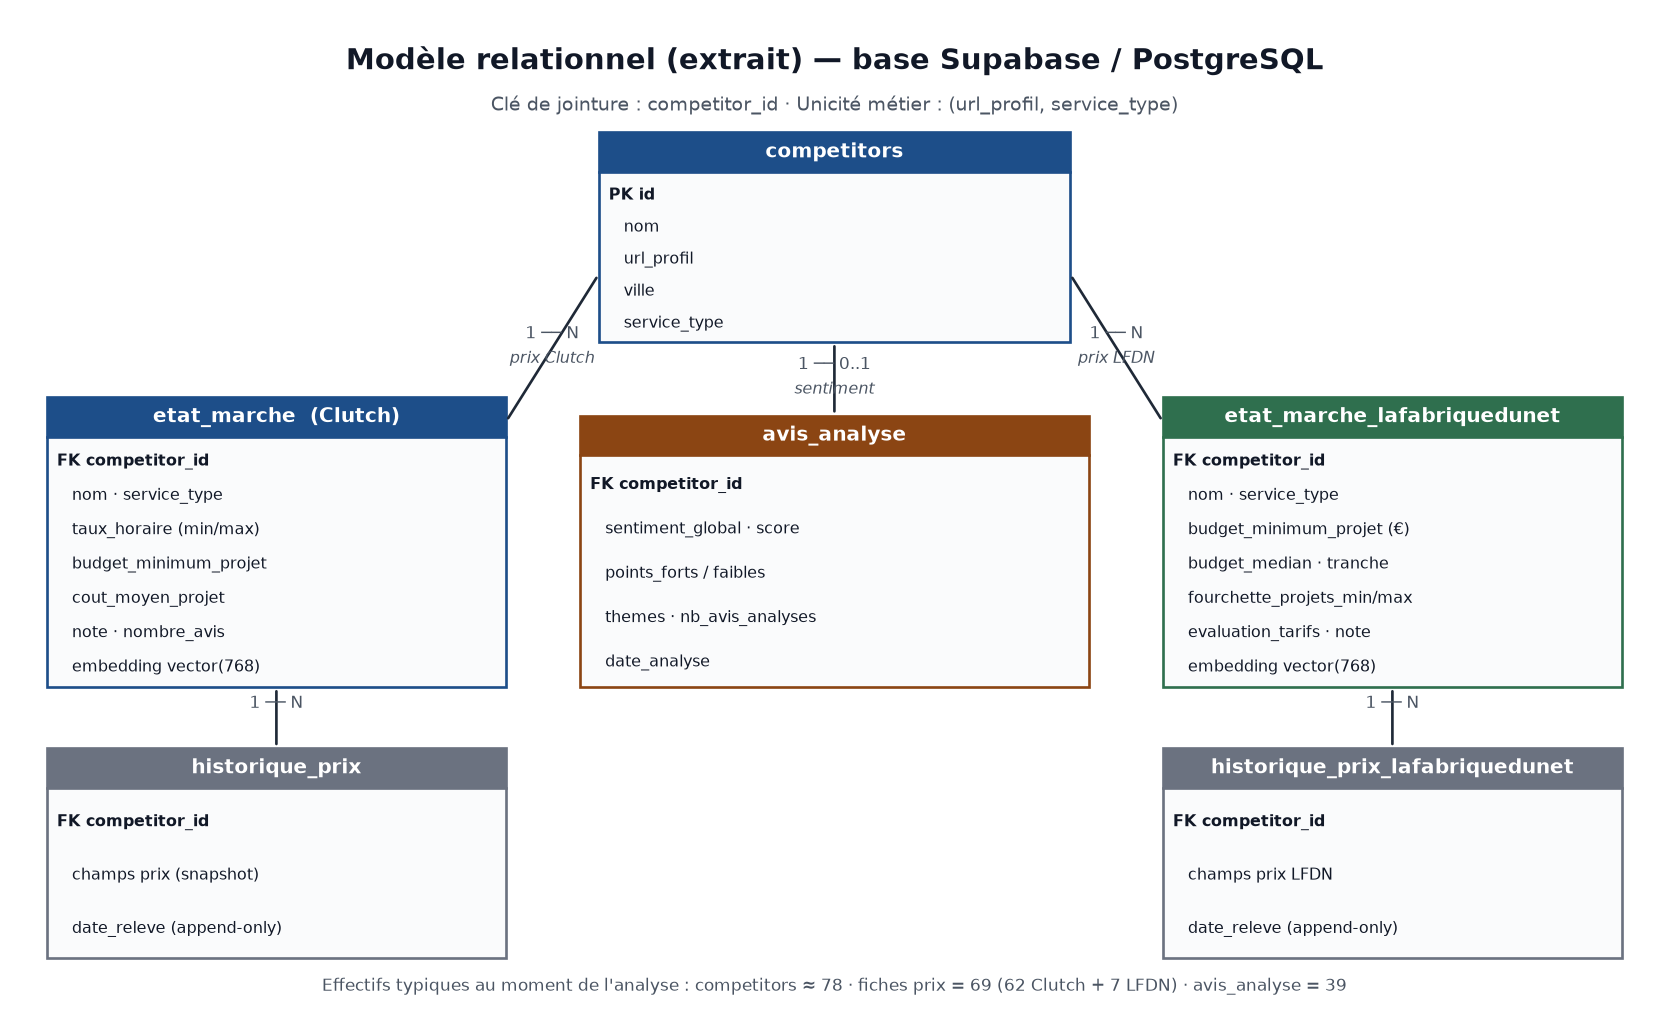
\includegraphics[width=0.95\textwidth]{img/modele_relationnel.png}
\caption{Modèle relationnel (extrait) de la base Supabase/PostgreSQL.
Tables principales~: \texttt{competitors}, \texttt{etat\_marche}, \texttt{etat\_marche\_lafabriquedunet}, \texttt{avis\_analyse}, \texttt{historique\_prix}.
Date du schéma~: 15/09/2026 (état de la base au moment de l'analyse).
Population représentée~: $78$ identités dans \texttt{competitors}~; $69$ fiches prix ($62$ Clutch + $7$ La Fabrique du Net)~; $39$ analyses d'avis.
Exclusion / non représenté sur le schéma simplifié~: tables annexes de monitoring non nécessaires à la lecture du RAG.}
\label{fig:modele_relationnel}
\end{figure}

\subsection{Analyse exploratoire des données (EDA)}

Sur les 78 entreprises identifiées (mobile et web confondus), 69 (88\,\%) disposent d'au moins une
donnée de prix exploitable. Parmi ces 69, 39 (56.5\,\%) disposent en outre d'une analyse de sentiment
fondée sur des avis clients en nombre suffisant. Cet écart de couverture entre identité, prix et
sentiment reflète le filtrage qualité décrit en section 10.1 : certaines entreprises ont été exclues à
une étape parce que leurs données étaient trop incomplètes pour être exploitées de façon fiable à cette
étape précise, sans être nécessairement exclues des étapes précédentes.

La distribution des taux horaires minimums (Clutch) fait apparaître une nette asymétrie vers le haut de
l'échelle plutôt qu'une répartition centrée (Figure~\ref{fig:distribution_taux_horaire}) : le mode se
situe dans la tranche 100--149 \$/h, qui concentre à elle seule 22 des 43 agences web (51\,\%) et 6 des 19
agences mobile (32\,\%). Les profils mobile et web diffèrent sensiblement sur ce point : le mobile est
proportionnellement plus représenté dans les tranches basses et moyennes (25--99 \$/h, 11 agences sur 19,
soit 58\,\%), tandis que le web bascule plus nettement vers le haut de la fourchette. Les positions
extrêmes restent rares dans les deux cas (une seule agence de chaque profil en dessous de 25 \$/h, et une
seule au-delà de 140 \$/h), ce qui situe l'essentiel du marché observé entre 25 et 150 \$/h. Les
statistiques descriptives complètes par \texttt{service\_type} (moyenne, médiane, écart-type) sont données
par \texttt{rapport\_eda.md}.

La répartition du sentiment global issu de l'extraction LLM montre une très forte prédominance des avis
positifs (37 entreprises, 95\,\%) sur les avis négatifs (2 entreprises, 5\,\%) ; aucun avis n'a été classé
neutre sur cet échantillon (voir Figure~\ref{fig:repartition_sentiment}).

Mise en regard de la note déclarée par les clients (sur 5), la corrélation entre la note globale et le
score de sentiment attribué par le LLM est de $r = 0.16$ ($n = 22$, $p = 0.47$). Ce calcul porte
volontairement sur le sous-ensemble d'entreprises pour lesquelles la note \emph{et} les avis analysés
proviennent de la même source de référence, Clutch ou La Fabrique du Net --- et non sur des avis
collectés ailleurs (réseaux sociaux, Google, etc.), afin de comparer deux mesures homogènes issues d'un
même corpus d'avis plutôt que deux corpus distincts. Sur ces 22 entreprises, le nombre d'avis analysés
(\texttt{nb\_avis\_analyses}) est d'ailleurs très proche du nombre d'avis brut relevé par la plateforme
(\texttt{nombre\_avis}) --- par exemple 36 avis Clutch pour 37 avis analysés chez Redlab Agency, ou 51
pour 53 chez SolveIt --- confirmant que l'analyse de sentiment porte bien, pour ce sous-groupe, sur le
même corpus d'avis que la note affichée.

Cette corrélation, faible et non significative au seuil usuel de 5\,\%, doit être interprétée avec
prudence : le sous-échantillon retenu présente une variance structurellement réduite (notes comprises
entre 4.18 et 5.0, scores de sentiment entre 0.88 et 1.00), ce qui limite mécaniquement l'amplitude
d'une corrélation linéaire mesurable. Il faut par ailleurs souligner que \texttt{note = 0} dans
\texttt{etat\_marche} signifie l'absence d'avis sur la plateforme source (Clutch ou La Fabrique du Net),
et non l'absence totale d'avis pour l'entreprise concernée : 17 entreprises supplémentaires disposent
d'avis analysés (\texttt{nb\_avis\_analyses} > 0) issus d'autres sources, sans note de référence
comparable associée à ce même corpus, et sont de ce fait exclues du calcul de corrélation ci-dessus ---
un biais de sélection méthodologiquement assumé plutôt qu'une simple donnée manquante aléatoire.

Les deux indicateurs peuvent ainsi refléter des dimensions différentes de l'expérience client : la note
traduit une évaluation globale et explicite, tandis que le score de sentiment repose sur l'analyse
sémantique du contenu textuel de l'avis. Compte tenu du faible nombre d'observations et de l'absence de
significativité statistique, ce résultat ne constitue pas une validation directe de la fiabilité de
l'extraction zero-shot ; il met plutôt en évidence la complémentarité potentielle entre l'évaluation
quantitative déclarée et l'analyse qualitative automatisée des avis, ainsi que l'intérêt de traiter les
deux sources de notation comme des populations distinctes plutôt que comme un seul échantillon homogène.

\subsection{Visualisations et interprétations statistiques}

Les figures suivantes, produites par \texttt{analyse\_donnees.py}, illustrent les principaux résultats présentés précédemment. Pour chaque figure sont indiqués~: la date d'extraction des données, la population étudiée, les règles d'exclusion, ainsi que les effectifs ($n$) en complément des pourcentages.

\begin{itemize}
\item \textbf{Figure~\ref{fig:couverture_donnees}} --- Couverture des données par étape du pipeline (identité $\rightarrow$ prix $\rightarrow$ sentiment).
\item \textbf{Figure~\ref{fig:distribution_taux_horaire}} --- Distribution des taux horaires Clutch par type de service.
\item \textbf{Figure~\ref{fig:distribution_notes_source}} --- Distribution des notes globales par source.
\item \textbf{Figure~\ref{fig:repartition_sentiment}} --- Répartition du sentiment global issu de l'analyse LLM.
\item \textbf{Figure~\ref{fig:correlation_note_sentiment}} --- Corrélation entre note déclarée et score de sentiment LLM.
\end{itemize}

\begin{figure}[H]
\centering
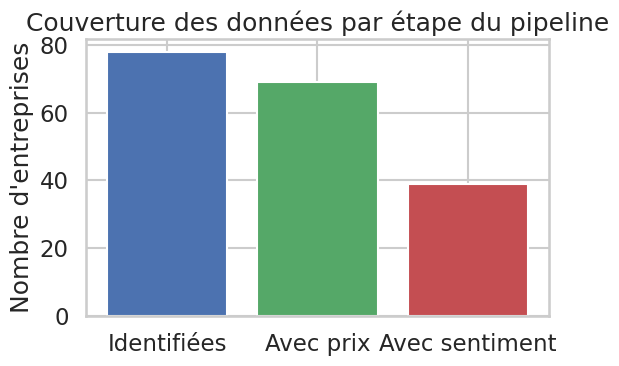
\includegraphics[width=0.8\textwidth]{img/couverture_donnees.png}
\caption{Couverture des données par étape du pipeline (identité, prix, sentiment).
Effectifs~: $78$ entreprises identifiées ($100\,\%$)~; $69$ avec prix exploitable ($88\,\%$)~; $39$ avec analyse de sentiment ($50\,\%$ des identifiées, $56{,}5\,\%$ des fiches prix).
Date d'extraction~: 15/09/2026.
Population~: ensemble des concurrents collectés (Clutch et La Fabrique du Net, profils web et mobile).
Exclusion~: $9$ entreprises sans donnée de prix exploitable ni avis utilisable (champs \textit{Undisclosed} / absence totale d'information).}
\label{fig:couverture_donnees}
\end{figure}

\begin{figure}[H]
\centering
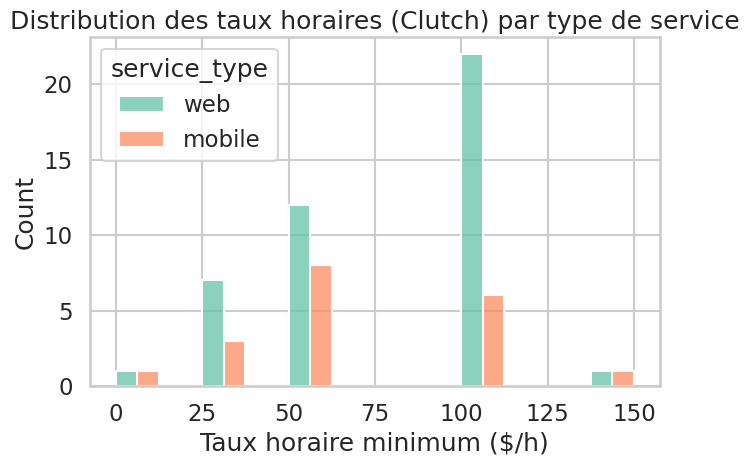
\includegraphics[width=0.8\textwidth]{img/distribution_taux_horaire.png}
\caption{Distribution des taux horaires Clutch par type de service (effectifs et pourcentages par tranche).
Mode~: tranche $100$--$149\,\$/\text{h}$ --- $22/43$ agences web ($51\,\%$) et $6/19$ agences mobile ($32\,\%$).
Date d'extraction~: 15/09/2026.
Population~: fiches Clutch avec taux horaire renseigné ($n_{\text{web}}=43$, $n_{\text{mobile}}=19$).
Exclusion~: entreprises La Fabrique du Net (pas de taux horaire)~; fiches Clutch sans taux horaire parseable~; valeurs \texttt{"No content available"} / \textit{Undisclosed}.}
\label{fig:distribution_taux_horaire}
\end{figure}

\begin{figure}[H]
\centering
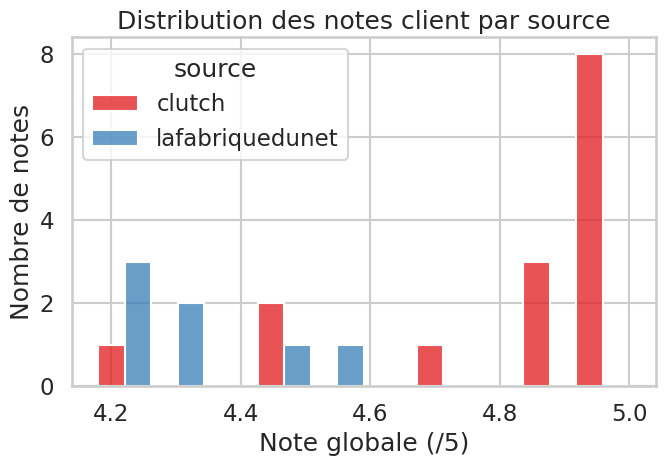
\includegraphics[width=0.8\textwidth]{img/distribution_notes_source.png}
\caption{Distribution des notes globales par source (effectifs $n$ et pourcentages par classe de note).
Date d'extraction~: 15/09/2026.
Population~: fiches dont la note source est renseignée et strictement positive (sous-ensemble de \texttt{etat\_marche} / \texttt{etat\_marche\_lafabriquedunet}).
Exclusion~: notes nulles ou absentes ($note = 0$ ou non renseignée), qui ne correspondent pas nécessairement à une absence d'avis hors source (cf.\ distinction avec \texttt{avis\_analyse}).}
\label{fig:distribution_notes_source}
\end{figure}

\begin{figure}[H]
\centering
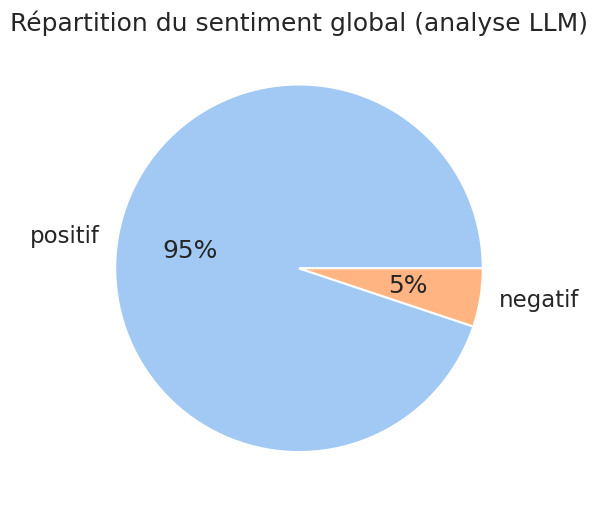
\includegraphics[width=0.8\textwidth]{img/repartition_sentiment.png}
\caption{Répartition du sentiment global issu de l'analyse LLM.
Effectifs~: positif $37$ ($95\,\%$)~; négatif $2$ ($5\,\%$)~; neutre $0$ ($0\,\%$)~; $n=39$.
Date d'extraction~: 15/09/2026 (date d'analyse des avis).
Population~: concurrents présents dans \texttt{avis\_analyse} ($n=39$).
Exclusion~: $30$ fiches prix sans analyse de sentiment (avis insuffisants ou non collectés).}
\label{fig:repartition_sentiment}
\end{figure}

\begin{figure}[H]
\centering
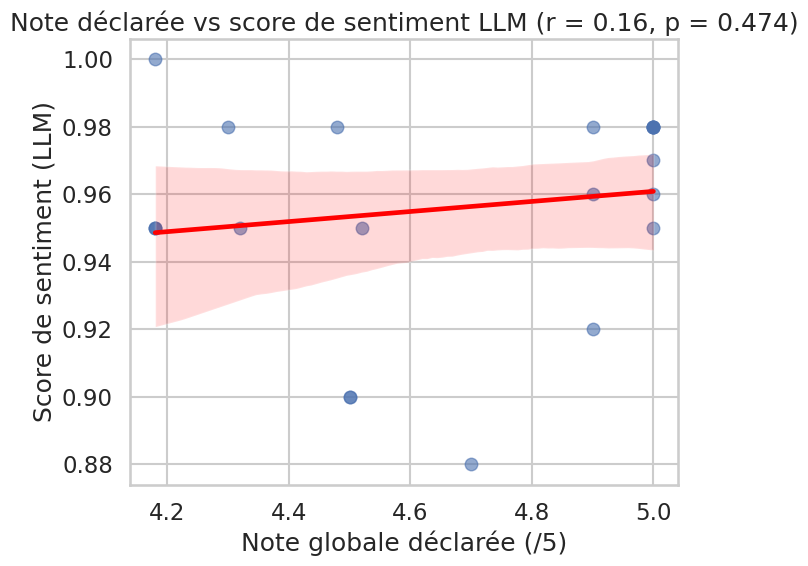
\includegraphics[width=0.8\textwidth]{img/correlation_note_sentiment.png}
\caption{Corrélation entre note déclarée et score de sentiment LLM ($r = 0{,}16$, $n = 22$, $p = 0{,}47$).
Date d'extraction~: 15/09/2026.
Population~: entreprises pour lesquelles la note \emph{et} les avis analysés proviennent de la même source (Clutch ou La Fabrique du Net), $n=22$.
Exclusion~: couples note/avis issus de sources hétérogènes~; entreprises sans note source ou sans score de sentiment.}
\label{fig:correlation_note_sentiment}
\end{figure}

\subsection{Réduction de dimension des embeddings (PCA, t-SNE)}

Les embeddings vectoriels calculés par le système de RAG (Gemini, 768 dimensions) constituent un objet
d'analyse naturel : ils sont censés capturer une notion de proximité sémantique entre profils de
concurrents, notion qui sous-tend directement la recherche par similarité cosinus utilisée en production
(section 4.2.3). Une projection en deux dimensions via PCA, puis via t-SNE, permet d'évaluer visuellement
si cette hypothèse se vérifie.

La PCA, projection linéaire, ne conserve que 21\,\% de la variance totale sur ses deux premières
composantes (Figure~\ref{fig:pca_embeddings}) --- un taux faible, mais attendu compte tenu de la
dimensionnalité élevée des embeddings (768D) : une projection 2D ne peut capturer qu'une fraction limitée
de la structure d'un espace de cette dimension, et ce chiffre doit être lu comme une limite de la
visualisation plutôt que comme une caractéristique des embeddings eux-mêmes.

Le nuage de points fait apparaître, visuellement, un clivage net en deux groupes selon l'axe principal de
la PCA. Avant d'attribuer cette séparation à une similarité sémantique entre profils d'agences --- ce qui
aurait constitué un argument de validation pour l'architecture RAG --- plusieurs facteurs de confusion ont
été systématiquement écartés par diagnostic croisé (coloration successive du nuage de points selon
différentes variables) : ni le \texttt{service\_type} (mobile vs web), ni la source de collecte (Clutch vs
La Fabrique du Net) ne permettent d'expliquer ce clivage, les deux catégories étant mélangées dans les
deux groupes.

En revanche, la présence ou l'absence d'avis clients (\texttt{note > 0} ou \texttt{nombre\_avis > 0})
explique la quasi-totalité du clivage observé (Figure~\ref{fig:pca_diagnostic_avis}) : les 22 entreprises
disposant d'avis clients se trouvent \emph{toutes} dans le groupe de droite, tandis que le groupe de
gauche est composé à 100\,\% (30/30) d'entreprises sans aucun avis. Le groupe de droite reste néanmoins
hétérogène, puisqu'il contient également 17 entreprises sans avis. Cette structure suggère que l'axe
principal de variance des embeddings reflète en grande partie la présence ou l'absence de contenu textuel
lié aux avis clients dans les champs utilisés pour construire la représentation vectorielle, plutôt qu'une
similarité intrinsèque de positionnement métier entre agences.

Le t-SNE, projection non linéaire optimisée pour préserver les voisinages locaux, fait apparaître une
structure plus fine que la PCA, avec en particulier un sous-groupe compact et isolé correspondant
exclusivement aux sept entreprises issues de La Fabrique du Net --- cohérent avec le fait que ces sept
entreprises disposent toutes d'avis clients (et se classent donc, comme attendu, dans le groupe "avec
avis" de droite en PCA), mais leur isolement encore plus marqué en t-SNE peut également refléter une
différence de langue du contenu source (profils rédigés en français pour La Fabrique du Net, en anglais
pour Clutch), un facteur de confusion supplémentaire qui n'a pas été formellement écarté ici et qui
constitue une limite à documenter.

Ce résultat doit donc être interprété comme un indice partiellement positif mais nuancé : les embeddings
capturent bien une structure exploitable en 2D, mais celle-ci est dominée --- pour son axe principal --- par
un artefact de complétude des données (présence/absence d'avis clients dans le texte source) plutôt que par
un signal de similarité purement métier entre concurrents comparables. Cette observation ne remet pas en
cause le fonctionnement du RAG en tant que tel, la similarité cosinus opérant en haute dimension (768D) où
d'autres axes de variance, non visibles sur cette projection 2D, peuvent porter un signal sémantique plus
pertinent ; elle invite cependant à la prudence dans l'interprétation purement visuelle de cette validation,
et suggère une piste d'amélioration future : exclure les champs liés aux avis de la construction de
l'embedding, ou les traiter séparément, afin d'isoler un signal de similarité de positionnement métier plus
directement exploitable pour la recherche de concurrents comparables.

\begin{figure}[H]
\centering
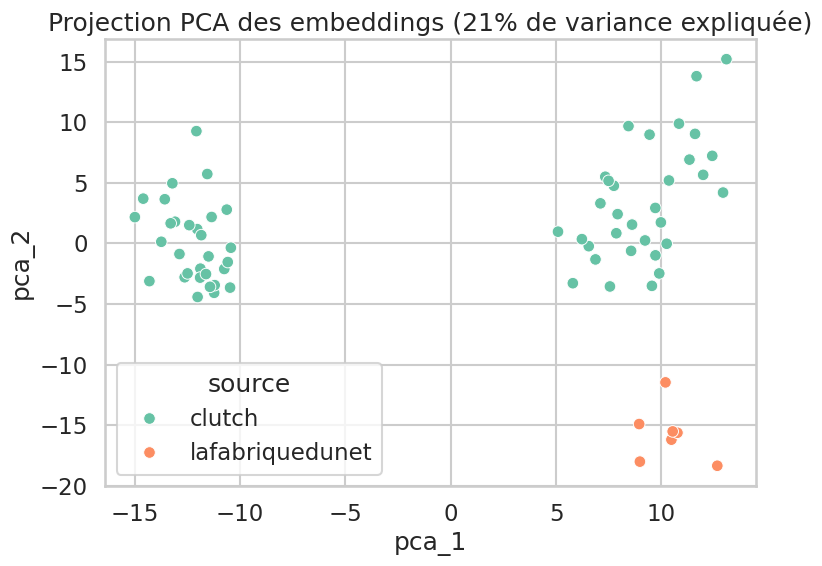
\includegraphics[width=0.8\textwidth]{img/pca_embeddings.png}
\caption{Projection PCA des embeddings, colorée par source ($21\,\%$ de variance expliquée sur les deux premières composantes~; $n=69$ fiches indexées).
Date d'extraction / indexation~: 15/09/2026.
Population~: embeddings Gemini (768 dimensions) des fiches présentes en base ($n=69$).
Exclusion~: concurrents sans embedding (aucun au moment de l'analyse)~; entreprises filtrées en amont ($78 \rightarrow 69$).}
\label{fig:pca_embeddings}
\end{figure}

\begin{figure}[H]
\centering
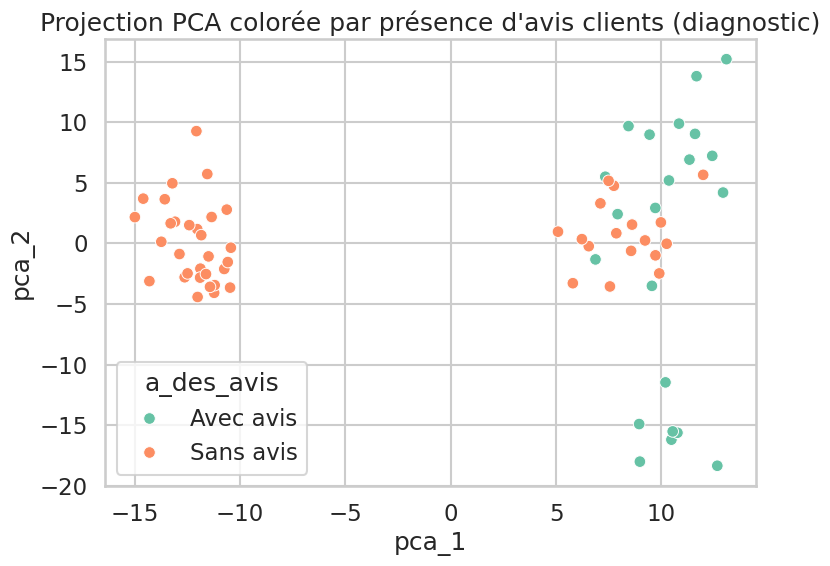
\includegraphics[width=0.8\textwidth]{img/pca_par_presence_avis.png}
\caption{Diagnostic PCA coloré par présence d'avis clients.
Effectifs~: groupe « avec avis » entièrement composé des $22$ entreprises ayant des avis source~; groupe « sans avis »~: $30/30$ ($100\,\%$) sans avis~; le groupe de droite reste hétérogène ($17$ sans avis également).
Date d'extraction / indexation~: 15/09/2026.
Population~: mêmes $n=69$ embeddings que la figure~\ref{fig:pca_embeddings}.
Exclusion~: idem~; coloration fondée sur $note > 0$ ou $nombre\_avis > 0$ dans les tables de prix.}
\label{fig:pca_diagnostic_avis}
\end{figure}

\begin{figure}[H]
\centering
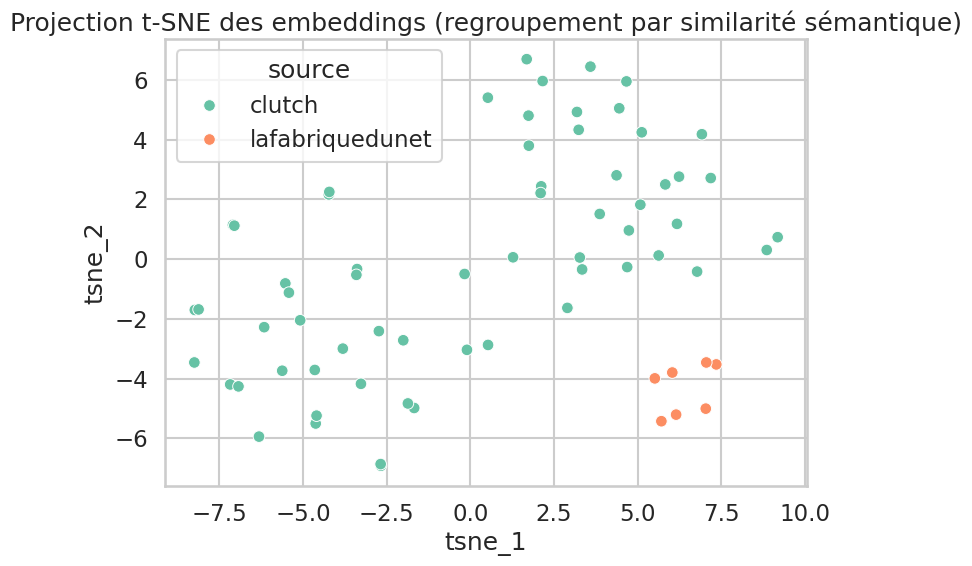
\includegraphics[width=0.8\textwidth]{img/tsne_embeddings.png}
\caption{Projection t-SNE des embeddings.
Sous-groupe isolé~: $7$ entreprises La Fabrique du Net ($100\,\%$ de cette source).
Date d'extraction / indexation~: 15/09/2026.
Population~: $n=69$ embeddings indexés.
Exclusion~: idem PCA~; interprétation prudente (artefact possible de langue FR vs EN du contenu source).}
\label{fig:tsne_embeddings}
\end{figure}
\newpage
% ============================================================
% Section « Modélisation et expérimentation » (version avec formules)
% Packages nécessaires dans le préambule :
%   \usepackage{amsmath, amssymb}
%   \usepackage{tabularx, setspace, float}
% ============================================================

\section{Modélisation et expérimentation}

\subsection{Architecture du système}

\begin{figure}[H]
\centering
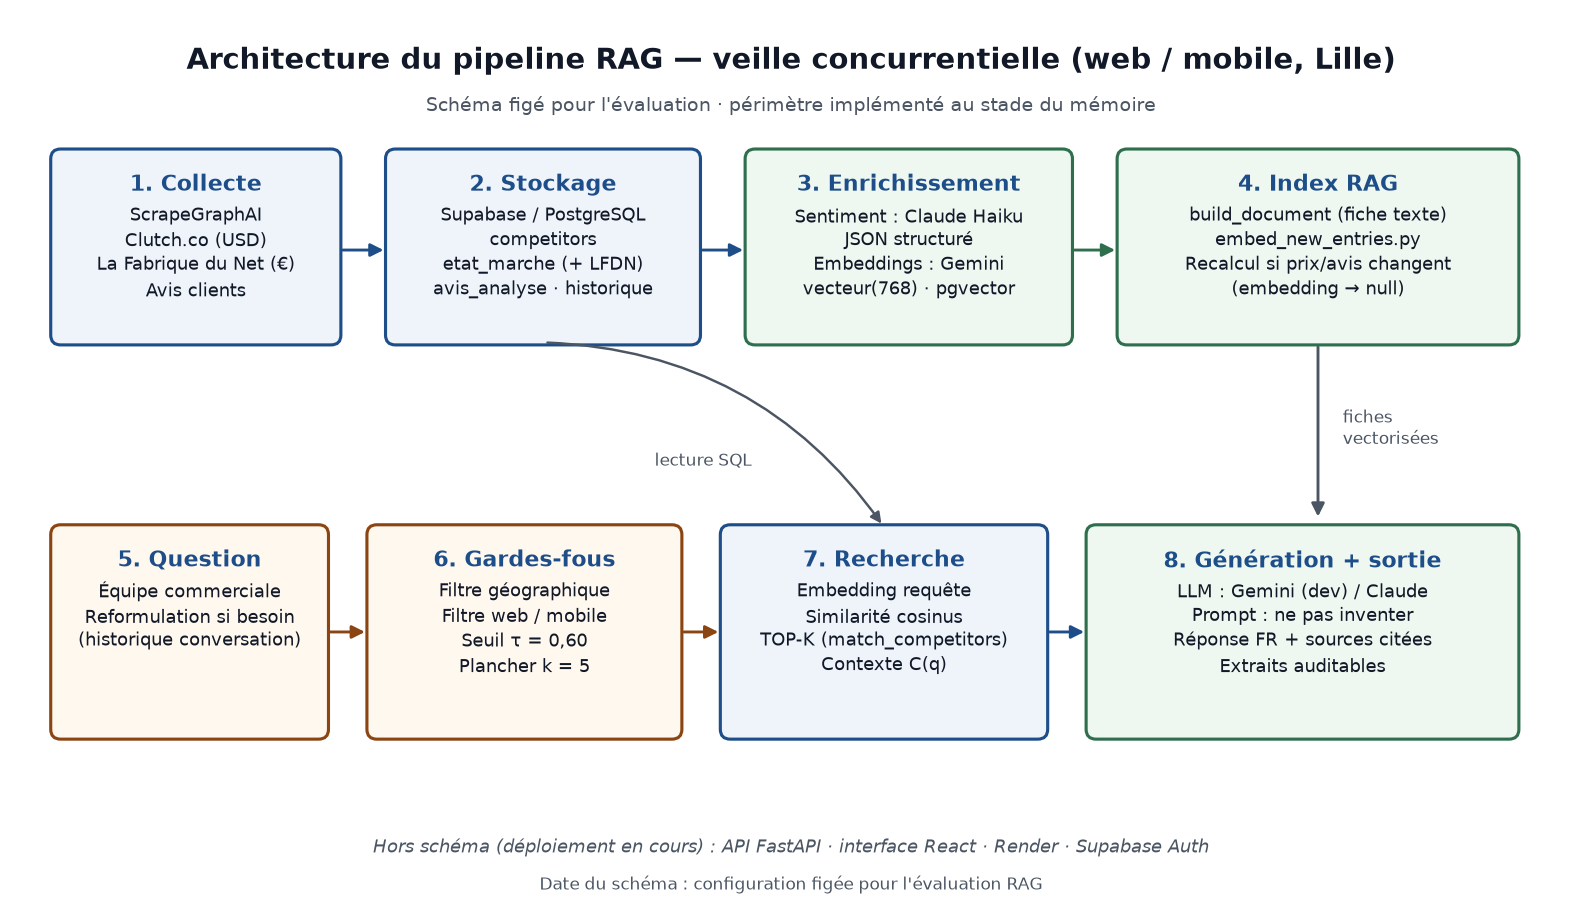
\includegraphics[width=0.95\textwidth]{img/architecture_rag.png}
\caption{Schéma d'architecture du pipeline RAG.
Flux~: collecte (ScrapeGraphAI) $\rightarrow$ stockage Supabase $\rightarrow$ analyse de sentiment (Claude) $\rightarrow$ embeddings (Gemini) $\rightarrow$ recherche vectorielle (\texttt{pgvector}) $\rightarrow$ génération de réponse (Gemini/Claude) $\rightarrow$ restitution sources.
Date du schéma~: configuration figée pour l'évaluation.
Périmètre~: composants effectivement implémentés au stade du mémoire (hors interface React/API FastAPI si non finalisées).
Exclusion~: services tiers non critiques (quota API, détails d'hébergement Render) omis pour la lisibilité.}
\label{fig:architecture_rag}
\end{figure}

\subsection{Pourquoi ce projet ne relève pas de l'apprentissage supervisé}

Le besoin exprimé par l'entreprise n'est pas de prédire une classe ou une valeur numérique. L'équipe
commerciale pose des questions en français sur ses concurrents : fourchettes de prix, avis clients,
comparaison entre offres web et mobile, informations sur une agence nommée. La réponse doit s'appuyer sur des
fiches déjà collectées et signaler explicitement les cas où ces fiches ne suffisent pas.

Un modèle de régression, de classification ou de clustering ajusterait ses paramètres $\theta$ en minimisant
une fonction de perte sur un jeu de données annoté $\{(x_i, y_i)\}_{i=1}^{n}$ :
\begin{equation}
    \hat{\theta} = \operatorname*{arg\,min}_{\theta} \; \frac{1}{n} \sum_{i=1}^{n} \mathcal{L}\big(f_{\theta}(x_i),\, y_i\big)
    \label{eq:supervise}
\end{equation}
Or un tel jeu n'existe pas : il n'y a ni centaines de questions étiquetées « bonne » ou « mauvaise »
réponse, ni avis annotés manuellement. Entraîner un modèle de langue, voire affiner un modèle comme
CamemBERT, aurait exigé des données et un temps de calcul que la durée du stage ne permettait pas. L'approche
retenue relève donc du \textit{transfert} : des modèles préentraînés, dont les paramètres $\theta$ restent
figés, sont appelés par API, et le travail de modélisation porte sur la manière de les articuler.

Le système construit est une architecture RAG (\textit{Retrieval-Augmented Generation}). Une question est
convertie en vecteur, comparée aux fiches des concurrents, puis un modèle de langue rédige la réponse à partir
des seules fiches retrouvées. Il n'y a donc aucune phase d'apprentissage des poids : le travail se décompose
en une phase de construction du pipeline, suivie d'une phase d'évaluation sur un jeu de questions fixé à
l'avance.

\subsection{Sélection des modèles}

Trois tâches ont été distinguées, car elles n'impliquent ni le même coût ni le même besoin de nuance.

\textbf{Recherche.} Chaque fiche concurrent est convertie en vecteur par le modèle
\texttt{gemini-embedding-2}, dont la dimension est fixée à 768 afin de rester alignée sur la colonne
\texttt{vector(768)} de Supabase. Deux modes d'utilisation du même modèle sont distingués :
\texttt{retrieval\_document} lors de l'indexation d'une fiche et \texttt{retrieval\_query} lors de
l'encodage d'une question. La comparaison repose sur la similarité cosinus, calculée par \texttt{pgvector} via
la fonction SQL \texttt{match\_competitors}.

Formellement, chaque texte $x$ (fiche ou question) est transformé par le modèle d'embedding en un vecteur
$\mathbf{e}(x) \in \mathbb{R}^{768}$. Lorsque la dimension est réduite de 3\,072 à 768 composantes, le vecteur
tronqué n'est plus de norme unitaire ; il est donc normalisé :
\begin{equation}
    \hat{\mathbf{e}}(x) = \frac{\mathbf{e}(x)}{\lVert \mathbf{e}(x) \rVert_2}
    \label{eq:norme}
\end{equation}
La proximité entre une question $q$ et une fiche $d$ est ensuite mesurée par la similarité cosinus :
\begin{equation}
    s(q, d) = \cos\big(\mathbf{e}(q), \mathbf{e}(d)\big)
    = \frac{\mathbf{e}(q) \cdot \mathbf{e}(d)}{\lVert \mathbf{e}(q) \rVert \, \lVert \mathbf{e}(d) \rVert}
    = \frac{\sum_{i=1}^{768} q_i \, d_i}
           {\sqrt{\sum_{i=1}^{768} q_i^{2}} \; \sqrt{\sum_{i=1}^{768} d_i^{2}}}
    \label{eq:cosine}
\end{equation}
avec $s(q,d) \in [-1, 1]$ ; plus la valeur est proche de 1, plus les deux textes sont sémantiquement proches.
L'avantage de cette mesure est qu'elle ne dépend que de l'angle entre les vecteurs, et non de leur norme. Pour
des vecteurs normalisés, elle se réduit au simple produit scalaire $s(q,d) = \hat{\mathbf{e}}(q) \cdot \hat{\mathbf{e}}(d)$.

Dans \texttt{pgvector}, l'opérateur \texttt{<=>} renvoie la distance cosinus
\begin{equation}
    d_{\cos}(q,d) = 1 - s(q,d)
    \label{eq:distance}
\end{equation}
et la fonction \texttt{match\_competitors} reconvertit ce résultat en similarité par $s = 1 - d_{\cos}$.

\textbf{Rédaction de la réponse.} Le modèle de chat est interchangeable. En développement,
\texttt{gemini-3.1-flash-lite} permet de limiter le coût et la consommation de quota. Pour la soutenance, le
même appel peut basculer vers Claude Sonnet (\texttt{claude-sonnet-4-5b}, 1\,000 jetons maximum) en
modifiant la variable \texttt{LLM\_PROVIDER}, sans changement dans le reste du pipeline.

\textbf{Analyse des avis, en amont du RAG.} Les avis ne sont pas traités par un classifieur entraîné. Claude
Haiku (\texttt{claude-haiku-4-5}) produit, en une seule passe et sans exemple annoté, un JSON au format imposé
comprenant le sentiment global, un score et des thèmes :
\begin{equation}
    \text{sentiment} \in \{\text{positif},\ \text{neutre},\ \text{négatif}\}, \qquad
    \sigma \in [0, 1], \qquad
    T \subseteq \mathcal{T}
    \label{eq:avis}
\end{equation}
où $\sigma$ est le score de sentiment et $\mathcal{T}$ la liste fermée des thèmes (délais, communication,
qualité, prix, réactivité, expertise technique). Un classifieur classique n'aurait fourni qu'une étiquette,
alors que l'objectif était de produire également des points forts et des points faibles directement
réutilisables dans la fiche.

Les tâches légères, comme la reformulation d'une question de suivi (« et pour le mobile ? ») ou le résumé de
l'historique de conversation, restent confiées au modèle Gemini le plus léger, même lorsque la réponse
finale est générée par Claude.

\subsection{Construction du système}

Le pipeline n'apprend pas : il prépare des documents, les indexe une fois pour toutes, puis les retrouve à
chaque question.

\subsubsection{Préparation et indexation des fiches}

Une fiche est un texte court construit par la fonction \texttt{build\_document}. Elle réunit le nom de
l'entreprise, le type de prestation (web ou mobile), la source (Clutch ou La Fabrique du Net), les tarifs
disponibles (budget minimum, taux horaire, coût moyen ou fourchette), puis au plus quatre points forts et
quatre points faibles issus de l'analyse des avis. Lorsque cette analyse n'existe pas, la fiche l'indique
explicitement. Le champ « thèmes », plus verbeux, n'est pas recopié : il répétait les informations déjà
présentes et alourdissait inutilement le contexte transmis au modèle.

Ces textes sont vectorisés une seule fois par le script \texttt{embed\_new\_entries.py}, et uniquement pour
les lignes dont l'embedding est vide. Tout changement de prix ou toute nouvelle analyse d'avis remet
l'embedding à \texttt{null}, ce qui déclenche un recalcul ciblé. Au moment de la question, le système ne
ré-encode donc jamais la base.

\subsubsection{Formalisation du traitement d'une question}

Soit $\mathcal{D}$ l'ensemble des fiches indexées. Pour une question $q$, le système construit un ensemble de
contexte $\mathcal{C}(q)$, puis le modèle de langue génère la réponse $r$ à partir de cet unique contexte :
\begin{equation}
    r \sim p_{\text{LLM}}\big(\,\cdot \mid q,\ \mathcal{C}(q)\big)
    \label{eq:rag}
\end{equation}
L'ensemble $\mathcal{C}(q)$ est obtenu en quatre temps.

\textbf{(i) Voisins les plus proches.} On classe les fiches par similarité décroissante,
$s(q, d_{(1)}) \ge s(q, d_{(2)}) \ge \dots \ge s(q, d_{(|\mathcal{D}|)})$, puis on retient les $K = 12$
premières :
\begin{equation}
    \mathcal{N}_{K}(q) = \big\{\, d_{(1)},\, d_{(2)},\, \dots,\, d_{(K)} \,\big\}
    \label{eq:topk}
\end{equation}

\textbf{(ii) Filtre web/mobile.} Soit $t(q) \in \{\text{web}, \text{mobile}\}$ le type de prestation détecté
dans la question, lorsqu'il est univoque, et $\operatorname{type}(d)$ celui de la fiche $d$ :
\begin{equation}
    \mathcal{N}'_{K}(q) =
    \begin{cases}
        \{\, d \in \mathcal{N}_{K}(q) : \operatorname{type}(d) = t(q) \,\} & \text{si ce sous-ensemble est non vide,} \\[4pt]
        \mathcal{N}_{K}(q) & \text{sinon.}
    \end{cases}
    \label{eq:filtre}
\end{equation}

\textbf{(iii) Seuil de similarité.} Avec le seuil $\tau = 0{,}60$ :
\begin{equation}
    \mathcal{S}(q) = \big\{\, d \in \mathcal{N}'_{K}(q) \;:\; s(q,d) \ge \tau \,\big\}
    \label{eq:seuil}
\end{equation}

\textbf{(iv) Plancher.} Avec $k = 5$ le nombre de fiches fournies au modèle :
\begin{equation}
    \mathcal{C}(q) =
    \begin{cases}
        \varnothing
        & \text{si } |\mathcal{S}(q)| = 0, \\[4pt]
        \text{les } k \text{ premières fiches de } \mathcal{N}'_{K}(q)
        & \text{si } 0 < |\mathcal{S}(q)| < k, \\[4pt]
        \text{les } k \text{ meilleures fiches de } \mathcal{S}(q)
        & \text{si } |\mathcal{S}(q)| \ge k.
    \end{cases}
    \label{eq:plancher}
\end{equation}
Dans le deuxième cas, les fiches ajoutées dont la similarité est inférieure à $\tau$ sont marquées
« confiance faible ». On note $\mathcal{F}(q) = \{\, d \in \mathcal{C}(q) : s(q,d) < \tau \,\}$ l'ensemble de
ces fiches ; le prompt précise que l'échantillon ne représente pas l'ensemble du marché dès que
\begin{equation}
    |\mathcal{F}(q)| > \frac{|\mathcal{C}(q)|}{2}
    \label{eq:faible}
\end{equation}

\subsubsection{Traitement d'une question à l'exécution}

À l'exécution, la fonction \texttt{ask} enchaîne cinq étapes.

\begin{enumerate}
    \item \textbf{Filtre géographique.} Si la question cite une ville connue hors de la zone couverte (Paris,
    Lyon, Tokyo, etc.) sans mentionner Lille ni les Hauts-de-France, la recherche s'arrête et un message
    indique que la base ne couvre pas cette zone. Ce filtre est volontairement incomplet : il complète la
    consigne du prompt sans la remplacer.
    \item \textbf{Recherche vectorielle.} La question est encodée, puis les 12 voisins les plus proches sont
    demandés à la base (équation~\ref{eq:topk}).
    \item \textbf{Filtre web/mobile.} Si la question porte clairement sur le web ou sur le mobile, et non sur
    les deux, les fiches de l'autre type sont écartées. Si ce filtre vide la liste, il est annulé
    (équation~\ref{eq:filtre}).
    \item \textbf{Seuil de similarité et plancher.} Les voisins dont la similarité cosinus est inférieure à
    0,60 sont écartés. S'il en reste au moins un mais moins de cinq, la liste est complétée jusqu'à cinq
    fiches, et ces compléments sont marqués « confiance faible ». S'il n'en reste aucun, la liste demeure
    vide : c'est le cas d'une question hors sujet, pour laquelle forcer des fiches produirait une réponse
    inventée (équations~\ref{eq:seuil} et~\ref{eq:plancher}).
    \item \textbf{Génération.} Les fiches retenues sont injectées dans un prompt qui interdit d'inventer,
    impose de signaler les informations manquantes et rappelle que la base porte sur le développement web et
    mobile à Lille. Si plus de la moitié des fiches sont en confiance faible (équation~\ref{eq:faible}), le
    prompt précise que l'échantillon ne représente pas l'ensemble du marché (69 fiches dans le texte du
    prompt).
\end{enumerate}

En conversation, une question de type « et lui ? » est d'abord reformulée à partir de l'historique, afin que
la recherche reçoive une phrase autonome. En l'absence de pronom ou de formulation en « et\ldots », la
question n'est pas réécrite.

\subsection{Paramètres retenus}

Il n'y a pas de validation croisée au sens statistique, puisqu'aucun poids n'est ajusté sur des plis. Les
réglages ont été fixés par essais successifs, en observant les questions pour lesquelles le système se
trompait.

\begin{table}[H]
\centering
\begingroup
\setstretch{1.1}
\small
\begin{tabularx}{\textwidth}{|p{4.2cm}|p{3.4cm}|X|}
\hline
\textbf{Paramètre} & \textbf{Valeur retenue} & \textbf{Rôle} \\
\hline
Dimension des vecteurs & $768$ & Aligne l'API et la colonne \texttt{pgvector}. Sans ce forçage, l'API renvoie
3\,072 dimensions. \\
\hline
Voisins demandés à la base ($K$) & $12$ & Laisse de la marge avant le filtre web/mobile et le seuil. \\
\hline
Nombre de fiches fournies au modèle ($k$) & $5$ & Assez pour comparer, sans noyer la réponse. \\
\hline
Seuil de similarité cosinus ($\tau$) & $0{,}60$ & En dessous, la fiche n'est pas considérée comme une vraie
correspondance. \\
\hline
Plancher & $k = 5$, seulement si $\lvert\mathcal{S}(q)\rvert \ge 1$ & Évite qu'une question large
(« la concurrence à Lille ») ne renvoie qu'un seul nom, sans rouvrir la porte aux questions hors sujet. \\
\hline
Jetons de la réponse Claude & $1\,000$ & Borne la longueur de la réponse commerciale. \\
\hline
\end{tabularx}
\endgroup
\caption{Paramètres retenus pour la configuration finale du pipeline RAG}
\label{tab:parametres}
\end{table}

Le seuil $\tau = 0{,}60$ est le réglage le plus sensible. Trop bas, une question sur la météo ou sur Tokyo
récupère malgré tout des agences, car les mots « prix » et « application » ressemblent à ceux des fiches.
Trop haut, une question générale ne ramène presque aucune fiche et donne l'impression que la base est vide.
Le plancher de cinq fiches ne s'applique que lorsqu'au moins une fiche dépasse le seuil, c'est-à-dire lorsque
$|\mathcal{S}(q)| \ge 1$ : c'est ce qui distingue une question vague mais pertinente d'une question hors sujet.

Le filtre géographique a été ajouté à la suite d'observations sur le jeu de
développement (19 questions). Sur une question du type « prix d'une application
mobile à Tokyo », la similarité restait élevée et le modèle respectait ou non
la consigne du prompt selon les exécutions. Le filtre par liste de villes rend
ce cas déterministe, sans appel au modèle. Ces ajustements (seuil, filtre)
ayant été réalisés après observation des échecs sur ce même ensemble de
questions, celui-ci est désormais traité comme un jeu de développement et non
comme un test final indépendant.

\subsection{Protocole d'évaluation}

\subsubsection{Séparation développement / test}

Deux jeux de questions sont distingués.

Le jeu de développement $Q_{\text{dev}}$ compte $|Q_{\text{dev}}| = 19$ questions.
Il a servi au réglage du seuil $\tau$, du filtre géographique et à l'analyse des
échecs. Il n'est plus utilisé pour rapporter les performances finales.

Le jeu de test indépendant $Q$ (cible $|Q| = 60$) est construit après figement
des modèles, prompts, filtres et paramètres. Les réponses et sources attendues
sont définies avant exécution. Il se répartit en familles :
\begin{itemize}
    \item $Q_{\text{pert}}$ : questions pertinentes (prix, sentiment, nominatives) ;
    \item $Q_{\text{hs}}$ : questions hors sujet, pour lesquelles aucune fiche
    ne doit être renvoyée ;
    \item questions hors zone géographique ;
    \item questions hors couverture métier (prestation ou information absente
    des fiches).
\end{itemize}

On note $Q_{\text{vt}} \subset Q_{\text{pert}}$ le sous-ensemble des questions
dont le concurrent attendu $d^{*}_q$ est connu à l'avance, et $\mathcal{C}(q)$
la liste des sources effectivement renvoyées pour la question $q$.

\subsubsection{Portée des métriques automatiques}

L'\textit{accuracy}, le score F1, l'AUC et la RMSE ne constituent pas les
métriques principales : il n'y a ni classe binaire apprise, ni erreur numérique
à minimiser. Les métriques calculées par \texttt{evaluate\_rag.py} diagnostiquent
le comportement de la recherche ; elles ne mesurent pas, à elles seules, la
véracité ni la complétude de la réponse générée.

\begin{itemize}
    \item \textbf{Comportement de retrieval attendu.} Pour une question
    pertinente, au moins une source est renvoyée. Pour une question hors sujet,
    aucune source. Pour une question hors zone, aucune source ou uniquement des
    sources sous le seuil. Pour une question hors couverture, aucune source ou
    une réponse indiquant explicitement que l'information n'est pas disponible.
    Si $b(q) \in \{0,1\}$ désigne cet indicateur :
    \begin{equation}
        \text{Comportement retrieval} =
        \frac{1}{|Q|} \sum_{q \in Q} b(q)
        \label{eq:comportement}
    \end{equation}
    Ce taux a une définition étroite : une source retournée ne prouve pas qu'une
    réponse est correcte. Un résultat de $100\,\%$ ne doit pas être assimilé à
    une exactitude générale du système.

    \item \textbf{Taux de questions pertinentes avec résultat.} Part des
    questions pertinentes pour lesquelles au moins une fiche est retrouvée
    (anciennement nommé « rappel », dénomination trompeuse ici) :
    \begin{equation}
        T_{\text{pert}} =
        \frac{\big|\{\, q \in Q_{\text{pert}} : |\mathcal{C}(q)| \ge 1 \,\}\big|}
             {|Q_{\text{pert}}|}
        \label{eq:taux_pert}
    \end{equation}

    \item \textbf{Taux de rejet des questions hors sujet.} Part des questions
    hors sujet qui ne ramènent aucune fiche. Ce n'est pas la précision de
    l'abstention :
    \begin{equation}
        T_{\text{rejet}} =
        \frac{\big|\{\, q \in Q_{\text{hs}} : \mathcal{C}(q) = \varnothing \,\}\big|}
             {|Q_{\text{hs}}|}
        \label{eq:taux_rejet}
    \end{equation}
    Lorsque $|Q_{\text{hs}}|$ est petit, le résultat demeure exploratoire.

    \item \textbf{Similarité moyenne.} Diagnostic de retrieval : moyenne des
    similarités cosinus des sources renvoyées :
    \begin{equation}
        \bar{s} =
        \frac{1}{\sum_{q \in Q} |\mathcal{C}(q)|}
        \sum_{q \in Q} \; \sum_{d \in \mathcal{C}(q)} s(q, d)
        \label{eq:sim_moy}
    \end{equation}

    \item \textbf{Hit Rate@$k$ et MRR.} Diagnostics de recherche sur
    $Q_{\text{vt}}$. Soit $\operatorname{rang}_q$ le rang de $d^{*}_q$
    ($+\infty$ s'il est absent) :
    \begin{equation}
        \text{Hit Rate@$k$} =
        \frac{1}{|Q_{\text{vt}}|}
        \sum_{q \in Q_{\text{vt}}}
        \mathbb{1}\big[\operatorname{rang}_q \le k\big]
        \label{eq:hitrate}
    \end{equation}
    \begin{equation}
        \text{MRR} =
        \frac{1}{|Q_{\text{vt}}|}
        \sum_{q \in Q_{\text{vt}}}
        \frac{1}{\operatorname{rang}_q}
        \label{eq:mrr}
    \end{equation}
    Le MRR (\textit{Mean Reciprocal Rank}) vaut 1 si la fiche est première,
    $1/2$ si elle est deuxième et 0 si elle est absente
    (avec la convention $1/{+\infty} = 0$). Ces indicateurs ne mesurent pas
    la véracité de la réponse générée.

    \item \textbf{Temps de réponse.} Durée totale $t_q$ d'un appel, embeddings
    et génération compris :
    \begin{equation}
        \bar{t} = \frac{1}{|Q|} \sum_{q \in Q} t_q
        \label{eq:temps}
    \end{equation}
\end{itemize}

La prudence de la réponse détectée par marqueurs lexicaux (« ne permettent pas »,
« aucune donnée », « ne mentionne pas », etc.) est une heuristique exploratoire :
une formule prudente peut accompagner une erreur, et l'échantillon concerné est
souvent réduit. Il ne s'agit pas d'un jugement humain portant sur chaque phrase.

\subsubsection{Grille d'évaluation humaine}

Pour évaluer le contenu, une grille humaine complète les métriques automatiques.
Pour chaque question, l'évaluateur note de 0 à 3 et justifie :
\begin{itemize}
    \item sources pertinentes retrouvées ;
    \item exactitude des montants et devises ;
    \item fidélité aux documents ;
    \item complétude ;
    \item abstention correcte ;
    \item utilité commerciale.
\end{itemize}
Les sorties brutes du système et les justifications sont conservées.

\subsection{Résultats}

\subsubsection{Campagne de développement (19 questions)}

Le tableau~\ref{tab:resultats-dev} rappelle la campagne menée sur le jeu de
développement, avec la configuration figée ($k = 5$, $\tau = 0{,}60$). Ces
chiffres documentent le réglage ; ils ne constituent pas l'évaluation finale
indépendante.

\begin{table}[H]
\centering
\begingroup
\setstretch{1.1}
\begin{tabular}{|l|c|}
\hline
\textbf{Métrique} & \textbf{Résultat (jeu de développement)} \\
\hline
Nombre de questions & $19$ \\
\hline
Comportement retrieval attendu
  (définition étroite) & $100\,\%$ \\
\hline
Taux de questions pertinentes avec résultat & $14/14$ ($100\,\%$) \\
\hline
Taux de rejet hors sujet & $3/3$ ($100\,\%$, exploratoire) \\
\hline
Similarité cosinus moyenne ($\bar{s}$) & $0{,}704$ \\
\hline
Hit Rate@5 (diagnostic recherche) & $80\,\%$ ($4/5$) \\
\hline
MRR (diagnostic recherche) & $0{,}800$ \\
\hline
Temps de réponse moyen ($\bar{t}$) & $8{,}25\,\text{s}$ \\
\hline
\end{tabular}
\endgroup
\caption{Résultats sur le jeu de développement ($|Q_{\text{dev}}|=19$).
Le taux de $100\,\%$ désigne uniquement le comportement de retrieval attendu,
et non une exactitude générale des réponses.}
\label{tab:resultats-dev}
\end{table}

Une seconde exécution sur le même jeu de développement donne les mêmes taux de
comportement retrieval, le même Hit Rate@5 et le même MRR. La similarité moyenne
passe à $\bar{s} = 0{,}693$ et le temps moyen à $\bar{t} = 9{,}92\,\text{s}$.
Les métriques de recherche sont donc stables ; la variation du temps de réponse
tient surtout à la latence des API et non à un changement de classement.

Le $3/3$ sur les questions hors sujet demeure exploratoire (échantillon
nominatif très réduit). Un Hit Rate de $80\,\%$ signifie que, pour l'une des
cinq questions nominatives, le concurrent attendu ne figure pas parmi les cinq
fiches retournées. Le MRR et le Hit Rate étant égaux, on peut en déduire que les
quatre fiches retrouvées le sont toutes au premier rang :
\begin{equation}
    \text{MRR} =
    \frac{1}{5}\left(\frac{1}{1} + \frac{1}{1} + \frac{1}{1} + \frac{1}{1} + 0\right)
    = \frac{4}{5} = 0{,}8
\end{equation}
Si l'une d'elles avait été au deuxième rang, le MRR aurait été inférieur au
Hit Rate. La similarité moyenne, proche de $0{,}70$, reste au-dessus du seuil
$\tau = 0{,}60$ : les fiches conservées ne sont pas des rapprochements limites.
Il s'agit d'un diagnostic de retrieval, pas d'une preuve de qualité
rédactionnelle.

Le temps de réponse, d'environ 8 à 10 secondes, est compatible avec un usage
commercial ponctuel, mais pas avec une saisie assistée au fil de la frappe.
La pause de trois secondes entre les questions du script d'évaluation n'est
pas comptabilisée dans ce temps : elle sert uniquement à rester sous le quota
gratuit de l'API.

\subsubsection{Évaluation finale indépendante}

Après figement de la configuration, le jeu de test indépendant ($|Q|=60$) est
exécuté sans nouvel ajustement de paramètres. Les métriques automatiques y sont
rapportées avec la même portée étroite (comportement de retrieval, taux de
questions pertinentes avec résultat, taux de rejet hors sujet, Hit Rate@$k$,
MRR, similarité moyenne). Elles sont complétées par la grille humaine décrite
ci-dessus ; les scores moyens humains et le détail des échecs par question sont
présentés avec les sorties brutes conservées.

% À compléter après le run complet sur les 60 questions :
% \begin{table}[H] ... \caption{Résultats sur le jeu de test indépendant} ...

\newpage
% \input{choixModèle}
% \newpage
% \input{deploiement}
% \newpage
% \input{conclusion_generale}
% \newpage

\pagenumbering{Roman}
\begin{thebibliography}{99}

\bibitem{beno2025}
Beno, J. P. (2025). \textit{ELECTRA and GPT-4o: Cost-Effective Partners for Sentiment Analysis}. arXiv:2501.00062.

\bibitem{lewis2020}
Lewis, P., Perez, E., Piktus, A., Petroni, F., Karpukhin, V., Goyal, N., Küttler, H., Lewis, M., Yih, W.,
Rocktäschel, T., Riedel, S., \& Kiela, D. (2020). Retrieval-augmented generation for knowledge-intensive NLP
tasks. \textit{Advances in Neural Information Processing Systems}, 33, 9459--9474.

\bibitem{simmering2023}
Simmering, P. F., \& Huoviala, P. (2023). \textit{Large language models for aspect-based sentiment
analysis}. arXiv:2310.18025.

\bibitem{springer2025}
Springer Nature (2025). \textit{Web Scraping for Competitive Intelligence: State of the Art and Case Study}.
Chapitre issu de link.springer.com/chapter/10.1007/978-3-032-01910-3\_2.

\bibitem{vamvourellis2025}
Vamvourellis, D., \& Mehta, D. (2025). \textit{Reasoning or Overthinking: Evaluating Large Language Models on
Financial Sentiment Analysis}. arXiv:2506.04574.

\bibitem{wu2024}
Wu, S., et al. (2024). \textit{Retrieval-Augmented Generation for Natural Language Processing: A Survey}.
arXiv:2407.13193.

\bibitem{xu2024}
Xu, Z., Cruz, M. J., Guevara, M., Wang, T., Deshpande, M., Wang, X., \& Li, Z. (2024). Retrieval-Augmented
Generation with Knowledge Graphs for Customer Service Question Answering. \textit{Proceedings of SIGIR
2024}, 2905--2909.

\bibitem{xue2024}
Xue, J., Zheng, M., Hu, Y., Liu, F., Chen, X., \& Lou, Q. (2024). \textit{BadRAG: Identifying Vulnerabilities
in Retrieval Augmented Generation of Large Language Models}.

\bibitem{yan2024}
Yan, S.-Q., Gu, J.-C., Zhu, Y., \& Ling, Z.-H. (2024). \textit{Corrective Retrieval Augmented Generation}.
arXiv:2401.15884.

\bibitem{yesuf2025}
Yesuf, Y., Fields, Z., Jain, A., \& Kassa, E. (2025). Artificial Intelligence Adoption as a Driver of
Innovation and Competitiveness in SMEs: A Bibliometric and Systematic Review. \textit{F1000Research}.
DOI:10.12688/f1000research.171494.1

\bibitem{yu2024}
Yu, H., Gan, A., Zhang, K., Tong, S., Liu, Q., \& Liu, Z. (2024). \textit{Evaluation of Retrieval-Augmented
Generation: A Survey}. arXiv:2405.07437.

\bibitem{bibliometrique2025}
Étude bibliométrique (2025). \textit{Combined use of web scraping and AI-based models for business
applications: research evolution and future trends}. ResearchGate.

\end{thebibliography}

\section*{Webographie}

\begin{itemize}
    \item \textbf{Clutch} --- plateforme de référencement et d'avis clients sur les agences de développement
    web et mobile, utilisée pour la collecte des taux horaires et des avis. \url{https://clutch.co}
    \item \textbf{La Fabrique du Net} --- comparateur d'agences web avec avis clients vérifiés, utilisé pour
    les fourchettes de prix par projet. \url{https://www.lafabriquedunet.fr}
    \item \textbf{Sortlist} --- plateforme de mise en relation entre entreprises et agences, utilisée comme
    source complémentaire d'avis clients. \url{https://www.sortlist.fr}
    \item \textbf{Google Avis} --- avis clients publiés sur les fiches Google Business des concurrents.
    \url{https://www.google.com/maps}
    \item \textbf{Trustpilot} --- plateforme d'avis clients vérifiés, utilisée comme source complémentaire
    d'avis. \url{https://www.trustpilot.com}
    \item \textbf{Topya} --- plateforme d'avis clients sur les prestataires de services numériques.
    \url{https://topya.fr}
    \item \textbf{Feedbax} --- plateforme de collecte d'avis clients, utilisée comme source complémentaire.
    \url{https://feedbax.fr}
    \item \textbf{ScrapeGraphAI} --- outil de scraping piloté par grand modèle de langage, utilisé pour la
    collecte automatisée des données de ce projet. \url{https://scrapegraphai.com}
    
\end{itemize}
\newpage
% \input{annexe}

\end{document}